\documentclass[letterpaper]{article}
\usepackage{natbib,alifeconf}
%Graphics package
\usepackage{graphicx}
\DeclareGraphicsExtensions{.png,.jpg,.pdf}
%For multirow feature to draw tables
\usepackage{multirow}
%Middle allignment in tables.
\usepackage{array}
%For Mathematics
\usepackage{amsmath}
\numberwithin{equation}{section}
%Float package used to specify positioning
\usepackage{float}
%Depth of upto four in sections.
%\setcounter{secnumdepth}{3}
\usepackage{algorithmic}
\usepackage{algorithm}

%For hyper referencing
\usepackage[colorlinks={true},linkcolor={black},citecolor={black},urlcolor={black}]{hyperref}
%In case you use the package hyperref to create a PDF, the links to tables or figures will point to the caption of the table or figure, which is always below the table or figure itself. Therefore the table or figure will not be visible, if it is above the pointer and one has to scroll up in order to see it. If you want the link point to the top of the image you can use the package hypcap with:
\usepackage[all]{hypcap}

\usepackage[acronym]{glossaries}
\makeglossaries
\newacronym{al}{AL}{Artificial Life}
\newacronym{ca}{CA}{Cellular Automata}
\newacronym{cas}{CAS}{Complex Adaptive System}
\newacronym{ea}{EA}{Evolutionary Algorithm}
\newacronym{ec}{EC}{Evolutionary Computation}
\newacronym{ep}{EP}{Evolutionary Programming}
\newacronym{es}{ES}{Evolutionary Strategies}
\newacronym{formal}{FormAL}{Formal Artificial Life}
\newacronym{ga}{GA}{Genetic Algorithm}
\newacronym{gp}{GP}{Genetic Programming}
\newacronym{rna}{RNA}{Ribonucleic Acid}

\title{Modeling the Evolution of Mimicry}
\author{Mohiul Islam$^{1}$ \and Peter Grogono$^{1}$ \\
\mbox{}\\
$^1$Concordia University  \\
moh\_i@encs.concordia.ca \\
grogono@cse.concordia.ca}


\begin{document}
\maketitle

\begin{abstract}
A novel agent based, artificial life model, for the evolution of mimicry is presented. This model is a predator-prey co-evolution scenario where pattern representation phenotype is simulated with Cellular Automata, while behaviors of pattern recognition is configured with Hopfield Network. A visual three dimensional toroidal cube is used to construct a universe in which agents have complete freedom of mobility, genetic representation of behavior and reproduction capability to evolve new behaviors in successive generations. These agents are classified into categories of predator and prey species. Genome of prey species control their mobility and palatability, while 2D Cellular Automata (CA) is used to represent a pattern, where the rule to generate the CA is also genetically represented. Through evolution, successive generations of prey species develop new patterns to represent them both visually and to the predators. Predators are agents with the primary purpose of providing selection pressure for the evolution of mimicry. They are equipped with Hopfield Network memory to recognize new CA pattern and make intelligent decisions to consume the prey based on their level of palatability. Using the above construction of ideas, successful emulation of the natural process of mimicry is achieved. Also complex behavior pattern of Batesian and Mullerian mimicry is simulated and studied.
\end{abstract}

%Introductory Section
\section{Introduction}
\label{section:introduction}

%A few paragraphs are required to bring an appropriate introduction.
Mimicry is a process of deception. It is an evolutionary process with the help of which organisms survive by deceiving its predator. But this deception happens only if the environment contains similar appearing noxious organisms which the predators find unpalatable. Palatable organisms mimic the unpalatable ones through the process of evolution for survival of its species.

Artificial Intelligence is the field of computer science where scientists take concepts from psychology and implement into computer science. In contrast to that, in Artificial Life scientist take concepts from biology, specially evolutionary biology and genetics and implement into computer science. 

Christopher G. Langton is considered as one of the founders of the field of Artificial Life. He invented the term while organizing the first `\textsl{International Conference on the Synthesis and Simulation of Living Systems'} at the Los Alamos National Laboratory in 1987.

In defining Artificial Life Langton states the following,

\begin{quote}
\textsl{`` `Art' + `Life' = Artificial Life: Life made by Man rather than by Nature. Our technological capabilities have brought us to the point where we are on the verge of creating `living' artifacts. The field of Artificial Life is devoted to studying the scientific, technological, artistic, philosophical, and social implications of such an accomplishment."}
\end{quote}

\gls{al} has been described by Taylor, also as a tool for biological inquiry \citep{taylor1993}. While providing a brief survey over different AL models he talks about \textsl{Wetware systems} which work at the molecular level, the \textsl{Software systems} which work at the cellular level and the \textsl{Hardware systems} which works at the organism level. \textsl{Wetware} artificial life systems are the most similar to natural life and indeed are actually derived from natural life. Most of the experiments are attempts to direct an artificial evolutionary process toward the production of \gls{rna} molecules with specific catalytic properties. The initial contribution of \textsl{software systems} in artificial life was from John von Neumann when he designed the first artificial-life model (without referring to it as such), the famous self-reproducing, computation-universal cellular automata \citep{neumann1966}. He tried to understand the fundamental properties of living systems, especially self-reproduction and the evolution of complex adaptive structures, by constructing simple formal systems that exhibit those properties. \textsl{Hardware systems} at the organism level can deal with an organism's sensory and nervous system, its body and its environment. Even though an organism's nervous system is usually considered as fantastically complex, the other interesting complex components can be its geometric, mechanical, dynamical or thermal properties. 

\subsubsection{Complex Adaptive System}
\label{subsubsec:complex-adaptive-system}
\gls{cas} are special cases of complex systems. They are complex as they are diverse and made up of multiple interconnected elements and adaptive as they have the capacity to change and learn from experience. Examples of complex adaptive systems include the stock market, social insect and ant colonies, the biosphere and the ecosystem, the brain and the immune system, the cell and the developing embryo, manufacturing businesses and any human social group-based endeavor in a cultural and social system such as political parties or communities. This includes some large-scale online systems, such as collaborative tagging or social bookmarking systems.

\subsubsection{Echo}
\label{subsubsec:echo}
Echo is a class of simulation model for complex adaptive system, designed primarily for gedanken experiments rather than precise simulations. Echo provides a population of evolving, reproducing agents distributed over a geography, with different inputs of renewable resources at various sites. Each agent has simple capabilities - offense, defense, trading and mate selection - defined by a set of chromosomes. Even though these capabilities are simple and defined simply, they provide a rich set of variations illustrating the four kernel properties of complex adaptive systems described in section \ref{subsubsec:complex-adaptive-system}.

\paragraph{Criteria}
Echo has been constructed based on a set of criterion. The following is a short summary on it extracted from Holland's \textsl{Hidden Order: How Adaptation Builds Complexity} \citep{holland1996}.

\begin{itemize}
	\item Simplicity is considered as the first and foremost criterion. Instead of emulating a real system Echo is more of a thought experiment. Simplicity is attained by carefully constraining agent interaction and also giving the agents only a primitive internal model. 
	\item Actions and interaction of each agent in echo has been designed to be part of a wide range of \textsl{CAS} setting. Their mobility is also part of a wide range of geographical setting. Input to the environment which is considered as a stimuli or resource, can also be diversified.
	\item Fitness of each agent, is an evolving criterion. Instead of considering fitness as an external exogenous factor, it should be dependent on the context provided by the site and other agents. The fitness value, instead of being a constant should evolve along with the system. 
	\item \textsl{``The primitive mechanisms in Echo should have ready counter parts in all \textsl{CAS}"}. Interpretation of results from the Echo model should be direct and ready-made. As simulation is nothing but manipulation of numbers and symbols, it is always possible to make fanciful and deceiving interpretation of them, taking the opportunity to prove one's point. So by applying primitive mechanism for interpretation it is possible to avoid misinterpretation. Another advantage is with the help of interpretations, selected mechanisms can be shown to be sufficient to generate the phenomenon of interest. Even though simulation cannot establish that a given mechanism is actually present, but it can establish its sufficiency or plausibility.
	\item The architecture of the Echo model should be flexible enough so that other well-studied mathematical models of particular \textsl{CAS} can be incorporated whenever required. Among other models the significant ones include, Dawkins' \textsl{biological arms race} \citep{dawkins1990} and Brower's \textsl{survival of mimics} \citep{brower1988} from ecology; Wicksell's \textsl{Triangle} \citep{marimon1989} and \textsl{overlapping generation models} \citep{anderson1989} in economics; the \textsl{prisoner's dilemma game} \citep{axelrod1984} in political science; Holland's \textsl{two-Armed bandits} \citep{holland1975} in operational research and Perelson's \textsl{antigen-body matching} \citep{perelson1999} in immunology. 
	\item As mathematical analysis provides the surest route to arrive at a valid generalization point, most aspects of the Echo model should be amenable to mathematical analysis. 
\end{itemize}

In developing Echo using the above set of criterion, a step by step approach has been taken. Among these steps of improvement, the work by Hraber titled ``The Ecology of Echo" \citep{hraber1997} is more from an ecological perspective and has been discussed in the following.

\paragraph{Organization}
As Echo is an agent-based model, it has a collection of agents distributed in a two dimensional site which contains resources. Agents in Echo have freedom and flexibility to move around in this environment. These agents are capable of replicating themselves, while also having the capability of making complex interactions. Interactions include combat, trading and mating.

\subparagraph{Resources and Sites}
Resource in a site of Echo form its very foundation. They are represented by letters (a,b,c,d). Everything in Echo is constructed by combining these letters as strings. These resources are treated much like an `atom' and by combining them as a molecular string, agents are constructed. Geographically, Echo is a collection of interconnected sites. Each site contains a fountain which is the source of resource for the agents in Echo. The amount of resource available in each site varies in time. A site with no resource can be compared to a `desert' while another site with increased availability of letters can be a water spring or a pond. 

\subparagraph{Agents}
\textsl{``Agents have a genome that is roughly analogous to a single chromosome in an haploid species"}. An agents \textsl{tag} is an external phenotype of its respective genotype (such as color). Agents have internal conditions or rules of interaction, which are genetically represented and they encode the agents internal preferences, behavioral rules and so forth. So interactions between multiple agents occur based on their conditions (rules for interactions) and tags (appearance). This results in sophisticated interaction between agents such as deception (mimicry, bluffing) and in-transitivities. \textsl{``The six (external) tag and (internal) condition genes possessed by every agent are the offense tag, defense tag, mating tag, combat condition, trade condition and mating condition"}. These genes are used to determine what sort of interaction between agents will take place and also the outcome of their interaction. 

Agents have two ways of reproduction, one being self replication, while the other is by interaction between a pair of agents. 

\subparagraph{Replication}
The replication process for agents is asexual reproduction. An agent needs to collect sufficient resource to start the self-replication process. After replication, the newly created agent receives a fraction of its parent's resource. Spontaneous mutation is applied to the gene for this process, where different mutation rate is applied to different parts of the gene. 

\subparagraph{Interactions}
There are diverse interactions between agents consisting of combat, trading and mating. Agents need to be in the same location in site for any interaction to take place. Testing for which selection of interaction to take place, is always conducted in the order of combat, trade and mating.

\subparagraph{Combat}
The interaction of combat is analogous to real world antagonistic behavior, where one agent is killed resulting in the survivor agent to receive all its resource. Depending on each agent's offense and defense tag and the tag prefixes, the winner is decided. A \textsl{combat matrix} is also calculated with the genome of individual agents, which helps in calculating the winner.

\subparagraph{Trading}
When two agents are chosen to interact and they do not engage in combat, they are given the opportunity to trade and mate. Trading and mating are very much a mutual agreement between agents compared to combat, which is more of a destructive process. \textsl{``Agents A and B will trade if A's trading condition is a prefix of B's offense tag and vice versa"}. Trading takes place for excess resources between agents, where excess is defined as the amount which the agent possess above the amount required for a replication process, plus some reserves. The value of the reserve is controlled with the help of a simulation parameter. A deceptive process is introduced here while trading takes place, when an agent might not have excess resource but will still be engaged in trade, as it is not possible for the other agent to know the resource of its opposite interactor. 

\subparagraph{Mating}
Only if two agents find each other suitable, they will engage in the mating process. Suitability for mating is decided on certain conditions based on the mating tag of individual agents. A form of two point crossover takes place to perform the mating action and produce diverse new agents. 

\paragraph{Discussion of Results}
The Echo model has good resemblance with natural ecosystem. It has stable patterns of interactions among genetic variants, or trophic networks. It consists of different levels of resources along with relative species abundance. Even different cataclysmic events such as meteor, drought and so fourth are introduced. Also several isolation effects are observed where a number of sites are allowed to evolve independently. In addition to that Echo contains interesting flow of resources. 

Two separate experiments are done with the above simulation to observe whether species abundance pattern can be used to find ecologically plausible behavior in Echo. To make a falsifiable comparison with biological systems, two ecological patterns are considered, each of which has similar quantitative properties in many different ecosystems that exist in nature. The objective is to compare these naturally occurring ecosystems with Echo. The ecological patterns are the Preston  curve and the species-area scaling relation. This allowed comparison of Echo diversity patterns with empirical patterns of species abundance.

Preston's canonical log normal distribution is the most widely accepted formalization of the relative commonness and rarity of species. The species-area scaling relation is also an important ecological pattern. The theory of island biography is predicted on species-area relations. In conservation biology, this relation has been used to predict the effects of different reserve size, with species diversity. Although the species-area relation can be derived from Preston's canonical log-normal distribution, a satisfactory explanation of the processes that regulate this relation has not been advanced. 

Now the question is, does Echo exhibit the robust ecological phenomenon of Preston curve and species area scaling relation? For Preston's curve plot, the data show, qualitatively the pattern of genome abundances in Echo population resembles the general patterns found in biological systems, although some differences are observed. But for species area curve some discrepancy was observed between the expected result and the observed values. Several factors were raised for this discrepancy. One was the choice of the simulation parameter. Second being the definition of different species in Echo as agents having different genome is considered from different species. Another factor being the balance between rates of speciation and extinction of population. 

Finally to answer the above question, it has been concluded that, Echo showed good quantitative agreement with naturally occurring species abundance distribution and species area scaling relation.

\section{The Inspiration: Mimicry}
\label{section:mimicry}

Henry W. Bates first published in 1862 his findings about the similarities and dissimilarities between Heliconiinae and Ithomiinae butterflies, after 10 years of research in the Brazilian rain forest. For the next hundred years, it simulated heated discussion among all groups of people, scientists, philosophers, theologians, teachers and amateur naturalists. Bates collected ninety-four pieces of butterfly. He grouped them according to their similar appearance. He found butterflies having similar appearance, exhibiting morphological features which point to completely different species even families. Out of the ninety four species, sixty seven are now classified as Ithomiinae, while twenty seven of them are Heliconiinae.

\subsection{Batesian Mimicry}
Even though Heliconiids are conspicuously colored, they are extremely abundant. They are also slow in mobility. Still predators in the surrounding area, mostly insectivorous birds do not prey on them, because of their inedible and unpalatable nature. Also because of this phenomenon other edible and palatable species such as ithomiinae and pieridae, pretend to be heliconiids and thus enjoy protection.

Repulsive animals, such as heliconiids are very conspicuously colored. Having this noticeable property, they are easily recalled by predators. Their wing pattern works as a warning to predators. Once a predator has the knowledge of their inedible and unpalatable property, they would probably never attempt to try it again. As this is true, if any organism within close family and species, but being edible and having a deceptive resemblance to those conspicuously colored species will be avoided by the predators. Wickler \citep{wickler1986} expresses,
\begin{quote}
\textsl{``Such unpalatable appearing and yet edible animals thus possess a false warning pattern, they `act a part'. An actor is a mime, and so the representation of a false warning pattern was called \textit{mimicry}. Since Bates was the first to point out this phenomenon, it has received the name \textit{Batesian Mimicry} in his honor."}
\end{quote}
In general, the animal which is avoided by predator for unpalatable behavior is called the \textbf{model} and the imitating animal is called the \textbf{mimic}.

\begin{figure}[h]
	\centering
	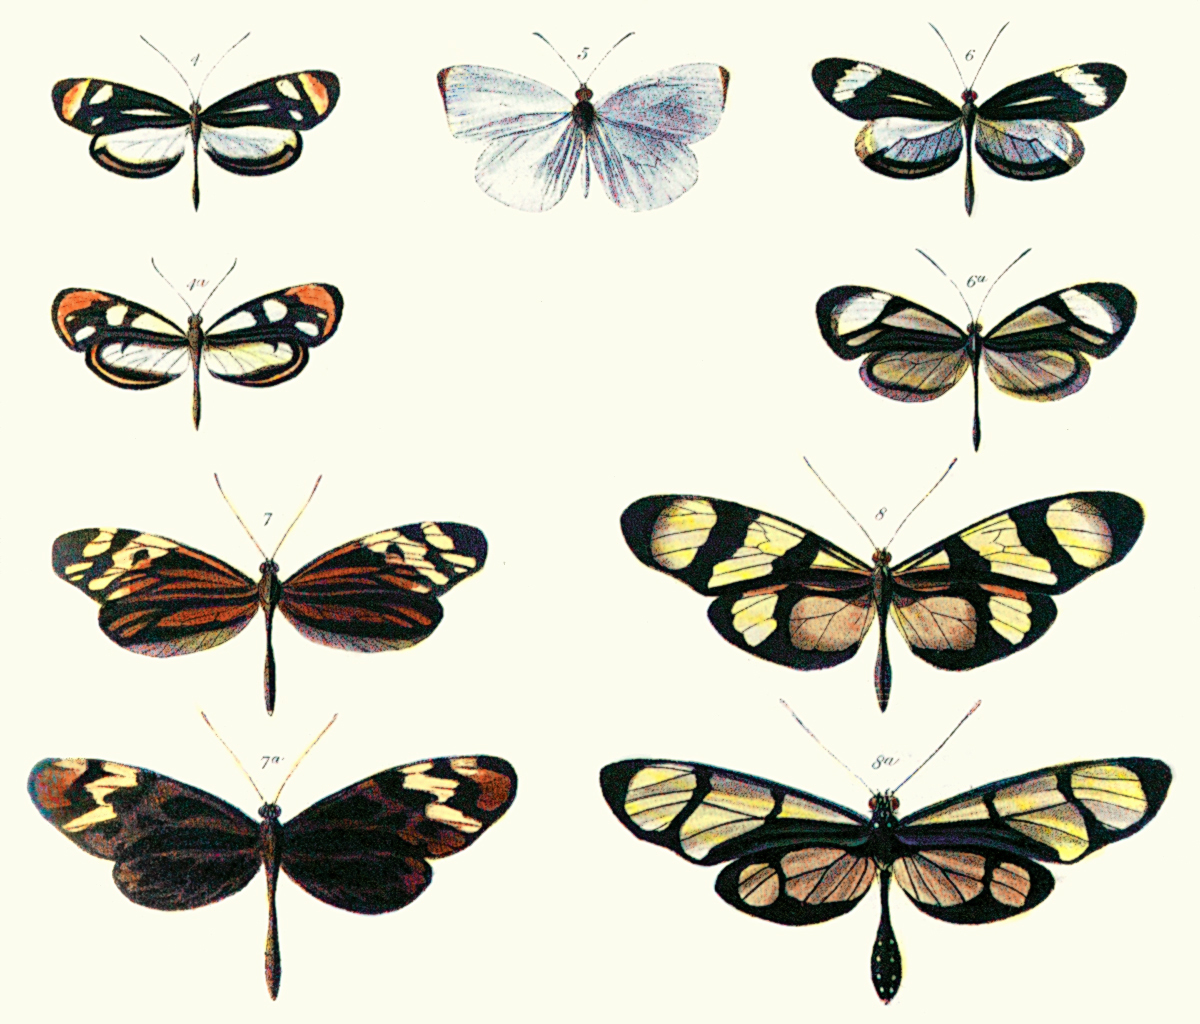
\includegraphics[width=0.5\textwidth]{../tex/images/Batesplate_ArM}
	\caption[Plate from Bates (1862) illustrating Batesian mimicry]{Plate from Bates (1862) illustrating Batesian mimicry between Dismorphia species (top row, third row) and various Ithomiini (Nymphalidae) (second row, bottom row). \citep{bates1862}}
	\label{fig:batesian-butterfly}
\end{figure}

\subsubsection{Definitions of Mimicry}
The best known definition of mimicry quoted to the present day, are those given by Wallace and listed in Poulton's \textit{The color of animals, their meaning and use} \citep{poulton1890colours}. The clauses are presented in the following:

\begin{itemize}
	\item \textsl{``that the imitative species occur in the same area and occupy the same station as the imitated".}
	\item \textsl{``that the imitators are always the more defenseless".}
	\item \textsl{``that the imitators are always less numerous in individuals".}
	\item \textsl{``that the imitators differ from the bulk of their allies".}
	\item \textsl{``that the imitation, however minute, is external and visible only, never extending to internal characters or to such as do not affect the external appearance."} 
\end{itemize}

According to Wickler \citep{wickler1986}, these five requirements, if fulfilled, indeed increase the probability that any given case of mimicry will be correctly diagnosed. But such supplementary clauses cannot be used as a definition of mimicry in general, though this is unfortunately often attempted. 

\subsection{Mullerian Mimicry}
\label{subsec:mullerian-mimicry}
Bates was not able to explain some phenomena of mimicry. Occasionally two inedible unrelated butterfly species are amazingly similar in appearance. An explanation for this was provided by Fritz Muller in 1878. Like Bates, Muller observed and caught butterflies in Brazil. When there are multiple inedible species it is hard for predators to recognize each of them to know which one to consume and which one to avoid. Because of predator's limited memory, all these species still lose their number even after being inedible. So to save this loss, and to prevent more sacrifice of their own kind, inedible species from different family also tend to evolve to have similar appearance. This phenomena is referred to as Mullerian Mimicry in the name of Fritz Muller.

According to Huheey \citep{huheey1988} \textsl{``Mullerian mimicry is normally viewed as a system of mutual warning coloration arising from the convergence of two or more warningly colored species, though two closely related species could also be Mullerian mimics through parallel evolution" \citep{muller1879}.} In Muller's view, predation load on each species are reduced when their warning signals are shared or converged. Naive young predators create the most impact in learning predation as they start their life with no knowledge or experience over the prey species. For cases like these, all unpalatable species should benefit from mutual advertising. If mutation gives opportunity for a single unpalatable prey to resemble a warningly colored species, it is expected to be more likely to survive predation than if the change was in opposite direction. Predators surviving on warningly colored species need to generalize; meaning if similar patterns signal unpalatability, predators recognition rate becomes much higher. Thus, variation in color pattern is tolerated, and mutations leading to even poor resemblance provides some protection. 

It is worth observing the fact that Mullerian mimicry is not deception, as it is to the predator's advantage to be able to recognize all deterrent and noxious species. Preys resemblance does not have to be close enough to cause misidentification on the part of the predator, but merely similar enough to remind it of a bitter past experience with similar prey. As Huheey continues \textsl{``Thus although there is selection for convergence to perhaps the most common, average pattern, or more likely the one associated with the most deterrence (both from the intensity of the traumatic stimuli and the frequency of predators receiving them), the convergence need not be rapid or precise. Indeed, the resemblance among Mullerian mimics is often not close, and the existence of very close mimics raises doubts that the mimicry is Mullerian."}

\begin{figure}[h]
	\centering
	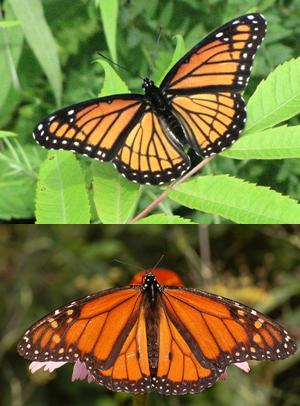
\includegraphics[scale=0.75]{../tex/images/BatesMimButter}
	\caption[A very well-known example of mimicry, the viceroy butterfly]{A very well-known example of mimicry is the viceroy butterfly (top) which has a pattern very similar to the unpalatable monarch butterfly (bottom). It was considered for a long time that this is an ideal example of Batesian mimicry. But recently Brower discovered that the viceroy is actually just as noxious as the monarch, making this a case of Mullerian mimicry. \citep{brower1991} Image source: \href{http://en.wikipedia.org/wiki/Mullerian_mimicry}{Wikipedia}}
	\label{fig:mullerian-butterfly}
\end{figure}

\subsection{Evolutionary Dynamics of Mimicry}
\label{subsec:evolutionary-dynamics-of-mimicry}
The dynamics of mimicry has been investigated by Turner \citep{turner1988}, where he states that the evolution of mimicry can be explained best by the process of punctuated equilibrium instead of phyletic gradualism. 

\paragraph{Punctuated Equilibrium}
In evolutionary biology, punctuated equilibrium is the theory which proposes that most sexually reproducing species will remain in an extended state called \textit{stasis} while experiencing little evolutionary change for most of their geological history. When evolution occurs it is localized in rare, rapid events of branching speciation, called cladogenesis. Cladogenesis is the process by which species split into two distinct species, rather than one species gradually transforming into another. Thus, \textsl{``punctuated equilibria is a model for discontinuous tempos of change (in) the process of speciation and the deployment of species in geological time" \citep{gould1977}}. 

\paragraph{Phyletic Gradualism}
In contrast to punctuated equilibrium, phyletic gradualism states that species continue to adapt to new environmental and biological selection pressures over the course of their history, gradually becoming new species. Phyletic gradualism holds that a species population changes gradually; that is there is no clear line of demarcation between an ancestral species and a descendant species unless a splitting (cladogenetic) event occurs or the gradually-changing lineage is divided arbitrarily. During this process, evolution occurs at a smooth, steady and incremental (but not necessarily constant and slow) rate on a geological time scale. 

On this issue Turner states,

\textsl{``According to punctuated equilibrium, therefore, evolution is not more or less both gradual and continual, as has been supposed for most purposes in most post-Darwinian theories. Rather, most morphological change is held to take place within geologically short periods, separated by vastly longer periods of comparative stasis \citep{eldredge1972}. The rapid, large changes all occur during speciation, that is to say during the branching of the evolutionary tree (cladogenesis);" \citep{turner1988}}

\begin{figure}[h]
	\centering
	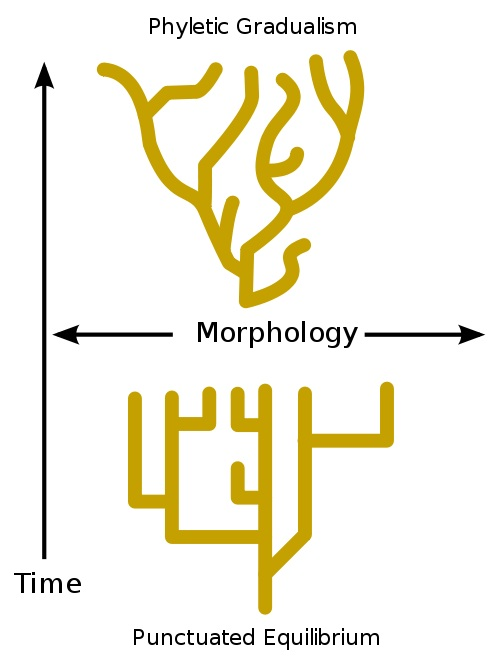
\includegraphics[scale=0.5]{../tex/images/Punctuated-equilibrium}
	\caption[Punctuated equilibrium vs. phyletic gradualism]{Punctuated equilibrium, bottom, consists of morphological stability and rare bursts of evolutionary change, while the top explains phyletic gradualism. Image source: \href{http://en.wikipedia.org/wiki/Punctuated_equilibrium}{Wikipedia}}
	\label{fig:punctuated-equilibrium}
\end{figure}

To explain the dynamic evolutionary process of mimicry, Turner came up with a synthetic theory \citep{turner1988}, which was originated by Poulton \citep{poulton1912} and Nicholson \citep{nicholson1927}, termed as the \textbf{two stage model}. This theory states that mimicry normally arises in two steps. A comparative large mutation achieves a good approximate resemblance to the model; it is followed by gradual evolutionary changes that refine the resemblance, in many cases to a high degree of perfection \citep{sheppard1972} \citep{ford1964}. This two-stage theory has been applied for the explanation of Mullerian mimicry as well.

\subsubsection{Mimicry Ring}
Any theory of Mullerian mimicry has to take into account the phenomenon of the coexistence of multiple mimicry rings. If we examine the local butterfly fauna in any area of the world, we will find that between all the aposomatic (warningly colored and defended) species present there are normally only a limited number of different patterns, normally far smaller than the number of species. Each cluster of species, all sharing a common pattern, is termed as Mullerian mimicry ring. Thus, in the rain forest of South and Central America, most of the long-winged butterflies (ithomiids, danaids, and heliconids) belong to one of only five different rings.

\paragraph{Formation of Mimicry Rings}
In regards to the formation of mimicry ring Turner \citep{turner1988} has given a theory which takes into account the level of protection of different rings of butterfly species and their difference in phenotypic warning patterns. Different level of variation of these two parameter can give us very different formation of mimicry ring evolution. The cases are considered below.

\begin{itemize}
	\item If we imagine two different rings of similar warning patterns in one single habitat, similar enough that the envelop of protection afforded to one gives some protection to the more extreme variant of the other (in a simplified language, suppose that predators that have sampled species A sometimes avoid the more extreme members of species B because they mistake them as A), then these two species are subject to natural protection for mutual convergence of their patterns. Eventually they will form a rather accurate Mullerian mimicry ring.
	\item By contrast, if the two species have patterns so dissimilar that predators encountering one never imagine that it might be the other (the envelop of protection do not overlap the other species' phenotype distribution), then there is no selection whatever for convergence, and the two patterns will remain distinct indefinitely.
 \item But mutations of color patterns are occurring all the time. Suppose that species B happens to produce a mutation whose pattern falls within the envelop of protection afforded to species A. The mimicry need not be perfect, but if it is good enough, the mutation will have an advantage and will spread. In this way species B may, by a single mutation, become a Mullerian mimic of species A; in other word species B may switch from one Mullerian mimicry ring to another. Clearly, if the mimicry is not perfect, the two patterns will then gradually converge, making the resemblance ever closer. 
\end{itemize}

Like Batesian mimicry, Mullerian mimicry can evolve in two stages: the mutational, one way convergence stage followed by the gradual, mutual convergence stage. It is worth mentioning that in the first stage only the less protected species can adopt the pattern of the better protected species; mutations in the other direction is not favored.

Mimicry is one of the most fascinating cases of evolutionary biology. This phenomenon has been studied extensively as infinite number of evidence exists in nature. One hundred years after Bates first clearly defined the concept, a review of literature listed 1,500 papers arguing for or against it. And this figure is more than 40 years old as it has been taken from Wilcker \citep{wickler1986}, published in 1968. It is almost impossible to survey all the known examples of Mimicry, and this would in any case be pointless. Then again many examples can be found in Cott's \textit{Adaptive Coloration in Animals} \citep{cott1957}.

%Chapter describing the model
\section{The Model: Evolution of Mimicry}
\label{section:model}

%Entire section until past work needs to be revised when the model has been fully described.
The objective of this thesis is to design an agent based artificial life model for simulating the natural process of the evolution of mimicry.

There are mainly two species of agents. These agents have properties and behavior similar to the \textbf{model}, the \textbf{mimic} and the \textbf{predator} in the evolution of mimicry. We represent evolution of pattern for the model and the mimic with the help of \gls{ca}. Cellular Automata can be easily represented by simple rules, which can be expressed as a binary string. The predator will be equipped with a Hopfield network \citep{hopfield1982}, to be able to have pattern recognition capability. The process of evolution will of course be running at the genetic level. 

The choice of Hopfield Network memory for a predator can be considered appropriate as the number of patterns which can be recognized by this network is inversely proportional to the accuracy of recall. As more patterns are memorized, Hopfield network tends to make more errors. This behavior will be appropriate for the simulation of Mullerian mimicry. Mullerian mimicry happens because of limited memory of the predators. Because of this limited memory, multiple inedible butterflies seems to converge to a single ring.

The environment is designed as three dimensional, while the space will be of toroidal nature. This idea has been taken from the \textsl{Laws and Life} project by Peter Grogono \citep{grogono2003}.

\subsection{Past Work}
Various models of mimicry has been simulated and explored. The model by Turner \citep{turner1996} and the mathematical model of Huheey \citep{huheey1988} tend to focus on the selective pressure on prey brought about by the particular learning abilities of the predator, and employ simple Monte Carlo or mathematical approaches.

Sherratt \citep{sherratt2002} provides an innovative perspective on the evolution of warning signals by considering co-evolving predator and prey populations. The model's predators are deterministic, in that they have a fixed behavioral strategy over their lifetime, and cannot learn from experience. For both cryptic and conspicuous prey, each predator has fixed policy of either attacking or avoiding.

The latest work on modeling evolution of warning signals and mimicry with individual based simulation is done by Franks and Noble. Their initial work \citep{franks2002} seems to focus on putting some conditions of mimetic evolution in an individual based model with multiple species preyed upon by a single abstract predator, where the appearance of each prey species can evolve but their palatability is fixed.

On 2003 \citep{franks2003} another model for the origin of mimicry ring has been proposed by Franks and Noble. Accordingly theory suggests that all Mullerian mimics in an ecosystem should converge into one large ring, while this convergence will be encouraged by presence of Batesian mimics. So an evolutionary simulation to observe the above mentioned phenomenon has been presented in this piece of work.

Franks and Noble continue to test the influence on mimicry ring evolution by Batesian mimics in their work on \citep{franks2004}. Usually mathematical models of mimicry has fixed prey coloration and appearances, which enables a comparison of predation rates to demonstrate the level of protection a mimic might be afforded. In this model prey colorations are free to evolve. This phenomenon is used to examine the effect of Batesian mimicry on Mullerian mimics and mimicry rings. 

\subsubsection{Models by Franks and Noble}
\label{subsubsec:models-by-frank-and-noble}
%Explain more about the first model by Franks and Noble
The \textbf{first} model by Franks and Noble \citep{franks2002} is where \textsl{``multiple species are preyed upon by a single abstract predator; the appearance of each prey species can evolve but their palatability is fixed"}. Each individual had a single gene: a value representing their external appearance or phenotype. The phenotypes are constrained to a ring of values from 1-20 (where 20 and 1 are neighbors). The distance of one phenotype from another represents their levels of similarity. 

A single abstract predator was modeled with a simple reinforcement learning system. The predator's experience of each phenotype was represented by a score, which would be maintained by probability to consume the next prey species depending on similarity or difference in phenotype. 

The existence of mimetic effect were measured with the initial and final distances between prey species' phenotypes. Three experiments were noted. Firstly, with one palatable and one unpalatable species. For this Batesian mimicry was evolved. For the second experiment, with two unpalatable species, Mullerian mimicry was evolved if the two prey species have some initial resemblance. Experiment 3 was carried out with two unpalatable and one palatable species, where the phenotype of the palatable species moved towards that of one of the unpalatable species, which is in other words Batesian Mimicry.

The \textbf{second} model by Franks and Noble \citep{franks2003} is based on two working hypothesis:

\begin{enumerate}
	\item \textsl{All of the Mullerian mimics in a given ecosystem should eventually converge into one large ring in order to gain maximum protection.}
	\item \textsl{If the Mullerian mimics do not converge into one large ring, then the presence of Batesian mimics could entice them to do so, by influencing the rings to converge.}
\end{enumerate}

Although there are many mathematical and stochastic models of mimicry in the biological literature, this model gives attention to the evolution of mimicry ring phenomenon from an artificial life perspective.

%\subsubsection{Model Description}
\paragraph{Prey}
Similar to the first model this also contains a population of prey species each having an appearance and palatability level. Different species of prey were each assigned a fixed palatability level on a scale between zero and one (least to most palatable), where 0.5 is neutrally palatable. Palatable species have values greater than 0.5, and unpalatable species have values lower than 0.5. Each prey species have used two genes with values compositely representing their external appearance or phenotype. Both of these genes were constrained to values from 1 - 200. The Euclidean distance of one phenotype from another represented their level of similarity.

\paragraph{Predator}
Similar to Turner's stochastic model \citep{turner_et_al1984},  predators were modeled with a Monte Carlo reinforcement learning system. The predator's experience of each phenotype was represented by an attack probability, which was initialized to ambivalence at 0.5. After eating prey of a particular phenotype, the predator would make a post-attack update of the relevant probability according to the palatability of the prey consumed. The predator would use its experience of different prey appearances to help it decide on whether or not to attack at the next opportunity.

In contrary to the stochastic model \citep{turner_et_al1984},  predators would generalize on the basis of experience. A set of probability formula was used to come up with the current probability to consume a prey species based on its palatability and the previous probability of consumption based on experience using generalization rate and the Euclidean distance between the experienced phenotype and the consumed prey phenotype. 

%Explain the results for the second model by Franks and Noble
\paragraph{Results}
According to the first experiment, which started with 20 unpalatable prey species, hypothesis 1 of a single large mimicry ring was not established. There was existence of multiple mimicry rings of very different frequency (population). Second experiment was carried out with some palatable species along with the unpalatable ones which was able to reach conditions of Batesian mimicry also with less mimicry rings, where hypothesis 2 borne out. It can be observed that,

\begin{quote}
\textsl{``The presence of Batesian mimics would provide positive selection pressure on mutants and would, therefore, increase the probability that they would evolve an initial resemblance to another unpalatable species. Also, Batesian pressure on mimicry rings has the potential to push one ring into the range of another, helping to bridge a large phenotypic difference between them." \citep{franks2003}}
\end{quote}

\subsection{FormAL Framework}
The \textsl{``FormAL framework"} is a collection of ideas and concepts taken from Peter Grogono's \gls{formal} project \citep{grogono2003} and are used to build a framework for modeling the evolution of mimicry. The primary goal of the FormAL project was ``\textit{To study the emergence of complexity}". While the principal behind it was ``\textit{not to include a variable in an agent unless the variable is genetically controlled (or, at least, genetically influenced)}". We will see that this principal was not completely established in simulating mimicry as it was not possible to come up with a genetic representation of Hopfield Network which was used as a pattern recognizer for the predator species. 

\subsubsection{Agents}
In FormAL, an \textbf{Agent} is a simulated organism. It is designed simply, but with the following qualities:

\begin{itemize}
	\item It has behaviors to be able to reproduce itself using genetic information.
	\item Capable of modifying the structure of genome between generations.
	\item Able to interact with other agents.
	\item And also to survive and reproduce in a challenging environment.
\end{itemize}

\subsubsection{Spatial representation of the environment}
The framework consists of a three dimensional visual environment where agents of the individual based simulation gets complete freedom of movement defined from their genetic representation. 

\paragraph{Space}
The space of the environment is a three-dimensional lattice of discrete points. The coordinate of each point in space is of the form \((x,y,z) \in \Sigma^3\), where \(\Sigma\) be the set \(\{0, 1, ..., S-1\}\). \(S\) is a universal constant being a small positive integer, which in this simulation has been kept at 20 (the value of the \(World Size\) parameter in table \ref{tab:environment-control-parameters}). 

\paragraph{Time}
Time, being an integer \( (t \geq 0) \), advances in discrete steps in the simulation, where at each step the agents update themselves. 

\paragraph{Cell}
The entire three dimensional toroidal environment is divided in multiple cells. A cell is a three dimensional cubical section of the hyperspace. Accordingly in table \ref{tab:environment-control-parameters} \(ISize\) is the parameter that controls the number of cells in the environment. The size of a cell is evaluated from the entire world size. And the total number of cell is calculated as \(ISize^3 = 216\).

\begin{table}[h]
\centering
\begin{tabular}{| p{1.5cm} | >{\centering} p{1.6cm} | p{4cm} |}
	\hline
		\textbf{Parameter} & \textbf{Value} & \textbf{Description} \\ \hline
		ISize & 6 & Number of cell in single dimension of the 3-D toroidal cube\\ \hline
		World Size & 20 & Size of a single dimension of the 3-D toroidal cube\\ \hline
		Cell Size & \( World Size\) / \(ISize \) & Size of each cell\\ \hline
		Total Number of Cells & \( ISize^3  = 216\) & Total number of cells in the environment\\ 
	\hline
\end{tabular}
\caption{Parameters to control the environment.}
\label{tab:environment-control-parameters}
\end{table}

\begin{figure}[h]
	\centering
	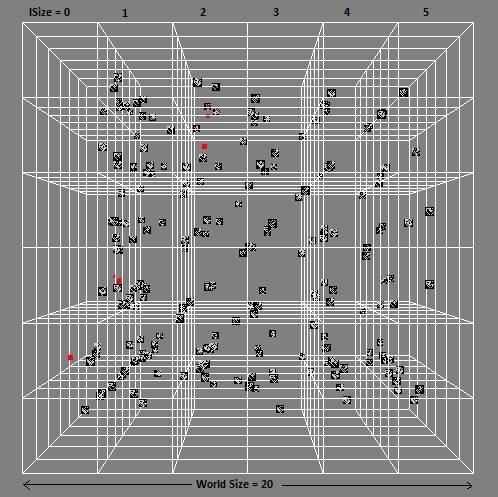
\includegraphics[width=0.5\textwidth]{../tex/images/cells-front}
	\caption[Three dimensional representation of the environment]{Three dimensional representation of the environment divided in cells. Presence of different species of agents inside.}
	\label{tab:3-d-environment-images}
\end{figure}

\subsubsection{Mobility}
An agent's position is calculated once during each step of update in time. The agents \(position\), \(force\), \(acceleration\) and \(velocity\) are all vector components. The \(force\) component is calculated from agent's mobility gene. And it is used to compute agent's \(acceleration\). If the \(force\) and \(velocity\) are both zero, then the agent has no effect in motion. Otherwise, Newton's law is used to obtain the \(acceleration\), which is integrated to obtain the new \(velocity\) and new \(position\).

\begin{algorithm}
	\caption{Algorithm for updating movement of the Agents}
	\label{algo:algorithm-movement-agents}
	\begin{algorithmic}
		\FOR{each step in time}
			\STATE $accelaration \gets ForceFactor * force - Friction * velocity$
			\STATE $velocity \gets DT*accelaration$ \COMMENT{DT is considered as Differential Time Set}
			\STATE $deltaPos \gets DT*velocity$
			\STATE $position \gets position + deltaPos$
		\ENDFOR
	\end{algorithmic}
\end{algorithm}

\begin{table}[h]
\centering
\setlength\tabcolsep{2pt}
\begin{tabular}{| p{1.5cm} | >{\centering} p{1cm} | p{5cm} |}
	\hline
		\textbf{Parameter} & \textbf{Value} & \textbf{Description} \\ \hline
		Force Factor & 40 & A unit vector is multiplied by this amount before being added to the force vector.\\ \hline
		Differential Time Step (DT) & 0.01 & The time step used for first-order integration of the motion equations.\\ \hline
		Friction & 5 & The friction constant used for motion calculations.\\ \hline
		Work Factor & 1 & \( Work done = WF * force * distance \), where \(WF\) is this constant.\\
	\hline
\end{tabular}
\caption{Parameters to control mobility of agents.}
\label{tab:mobility-control-parameters}
\end{table}

Algorithm \ref{algo:algorithm-movement-agents} explains the calculation of mobility of each agent at each time step of the simulation, while table \ref{tab:mobility-control-parameters} contains the values of the parameters used to apply to this algorithm.

\subsection{The Prey: Models and Mimics}

Only the significant characteristics which are required for a successful model of mimicry is implemented. As for this simulation we are considering heliconius butterfly, the representation of their wing pattern is with the help of cellular automata. So basically every prey organism will contain a genetic representation of cellular automata with which the predator will identify the prey and store its level of palatability in memory.

%More content needs to be added for cellular automata.
\paragraph{Cellular Automata}

Cellular automata are computer generated patterns applying very simple rules. First invented by Jon von Neuman and later extended by Stephen Wolfram, this field of study has created a lot of enthusiasm in the evolution of complexity with blocks of simplicity, in this case rules. We choose cellular automata as it can be easily represented with the help of a binary genome and then evolutionary operations on the genomic representation, such as mutation and crossover can easily be applied.

\begin{table}[h]
	\centering
	\setlength\tabcolsep{2pt}
	\begin{tabular}{| p{2.2cm} | c | c | c | c | c | c | c | c |}
	  \hline
	  Current Pattern & 111 & 110 & 101 & 100 & 011 & 010 & 001 & 000 \\ \hline
	  New state of center cell & 0 & 0 & 0 & 1 & 1 & 1 & 1 & 0 \\
	  \hline
	\end{tabular}
	\caption{Cellular Automata rule}
	\label{tab:cellular-automata-rule}
\end{table}

In generating the pattern of figure \ref{fig:cellular-automata-rule-30}, the genetic representation would be the `New state of center cell'. As figure \ref{fig:cellular-automata-rule-30} is a rule 30 cellular automata, the eight bit binary representation of 30 would be the genetic representation for this pattern. Generation of automata pattern from this binary string can be considered analogous to the complex pathway between the genotype and the phenotype that exists in all living organism.

\subsubsection{Species diversity}
\label{subsubsec:species-diversity}
Franks and Noble have used different models to diversify species. In \citep{franks2002} they have used linear difference in number ``constrained to a 'ring' of values  from 1-20 (where 20 and 1 are neighbors)" to distinguish species diversity. Here the distance of one phenotype from another represents their level of similarity. 

To use CA as prey pattern, an agent's genome is constructed as an 8 bit binary value with a decimal range between 0 to 255. Each of this 256 values have a unique CA pattern associated with it. When storing this pattern in Hopfield memory we take a linear representation of this 2-D pattern, while to consider similarity between two pattern we evaluate the hamming distance between their linear representation. 

With CA based pattern representation, population of prey species with a specific CA pattern can be grouped as one single species. And by restricting inter species reproduction we can control the diversity of patterns. But there is mutation applied when similar species mate with each other, so new species do born out of generations of existing species. So that is why we have two separate mutation rate while reproducing prey species. One being the ``Pattern Mutation Rate" (default values are mentioned in table \ref{tab:prey-control-parameters}) with which we control mutation of the first 8 bits of the genome while the ``Genome Mutation Rate" is used to control mutation of rest of the 9 bit genome (table \ref{tab:prey-genome}). Similar efforts of multiple mutation rate at varying location has been used in developing Echo as mentioned in section \ref{subsubsec:echo} \citep{hraber1997}.

\subsubsection{Genome}
The Genome of the prey species consists of 17 bits as presented in table \ref{tab:prey-genome}. The first eight bits represent the rule, which is used to generate Cellular Automata pattern. The next two bits are used to represent palatability of the organism explained detail in section \ref{subsubsec:genetic-palatability-representation}. The next six bits is the magnitude of the force with which mobility of the organism is calculated. The 17th bit is used to evaluate reproduction capability of the organism, depending on which the prey species is either capable or not capable to participate in reproduction.

\begin{table}[h]
\centering
\setlength\tabcolsep{2pt}
\begin{tabular}{|c|c|c|c|}
	\hline
		\textbf{Pattern(8)} & \textbf{Palatability(2)} & \textbf{Mobility(6)} & \textbf{Reproduction(1)} \\ \hline
		10101101					 	& 							01		 		 & 			110001					&					1						 		 \\ \hline
\end{tabular}
\caption{Distribution and purpose of each gene of the 17 bit prey genome.}
\label{tab:prey-genome}
\end{table}

\subsubsection{Reflection of punctuated equilibrium}
\label{subsubsec:reflection-of-punctuated-equilibrium}
Punctuated equilibrium has been defined in section \ref{subsec:evolutionary-dynamics-of-mimicry} as the evolutionary process that is more inclined to cladogenesis instead of gradualism. Also Turner \citep{turner1988} emphasizes on punctuated equilibrium to describe the evolution of mimicry instead of phyletic gradualism. The design of the model under discussion also follows Turner's explanation in terms of evolving mimicry. As it can be observed, new CA patterns evolve from existing ones in prey population just by a single mutation in the pattern gene. Mimics do not follow a gradual process of evolution to look close to models but rather the change happens randomly through a single step mutation. The mutations that are favored, helps the mimics to survive while the unfavored ones fail to persist. It can be observed later in table \ref{tab:diff-in-pattern} how CA patterns of prey species can have vastly different configuration for a unit change in their representative gene. 

\subsubsection{Genetic representation of palatability}
\label{subsubsec:genetic-palatability-representation}
The palatability of each prey species is fixed and has been represented with 2 bits of the genome giving it a range of 0 to 3 with four levels of palatability. The combinations are as follows:

\begin{table}[h]
	\centering
	\begin{tabular}{|c|c|}
		\hline
			\textbf{Gene (Index 8 to 9)} &	\textbf{Palatable} \\ \hline
			00									& True 			\\ \hline
			01									& True 			\\ \hline
			10									& False 		\\ \hline
			11									& False 		\\
		\hline
	\end{tabular}
	\caption{Genetic representation of palatability}
	\label{tab:genetic-representation-palatability}
\end{table}

This representation in table \ref{tab:genetic-representation-palatability} is unlike Franks and Noble \citep{franks2003} where palatability level has been used on a scale between zero and one (least to most palatable), where 0.5 is neutrally palatable. 

\subsubsection{Interaction between other Prey and Predators}
The prey have been defined to have many conglomerate behavior in the environment. Prey interaction with other prey species and with predators make the evolution of mimicry possible. Mobility of prey species and their reproduction capability are two important behaviors which result from interaction. 

\paragraph{Mobility}
The mobility genes of the prey consist of 6 bits. These six bits are used to calculate the force with which each prey try to move towards any neighborhood cell. The algorithm sorts all neighboring cell descending to the number of prey species. Then it selects the cell which contains the highest number of prey with zero predator. If all the neighboring cells contain predators, then the algorithm sorts the neighboring cells descending on the number of predators and chooses the one which contains the least. Algorithm \ref{algo:algorithm-movement-prey} explains in detail.

\begin{algorithm}[h]
	\caption{Algorithm for updating position of the Prey species}
	\label{algo:algorithm-movement-prey}
	\begin{algorithmic}
		\FOR{each step in time}
			\STATE $forceMagnitude \gets convertToDecimal(genome[10-15])$
			\STATE Get list of neighborhood cells, sorted by population of prey species.
			\STATE From the sorted cell list choose the one with the least number of predators and most number of prey.
			\STATE Move towards the selected cell with $forceMagnitude$ unit of force.
		\ENDFOR
	\end{algorithmic}
\end{algorithm}

\paragraph{Reproduction}
Every prey species starts reproducing when it reaches the \textsl{``Reproductive age limit"}. If it is capable of reproducing, which is decided based on its 17th bit gene, the prey will randomly select another prey species with similar pattern and palatability from the same cell and mate with it. Now the other prey also needs to be genetically capable of reproduction and needs to reach its age limit. A new genome is created from the existing genome of the two prey by applying single point crossover operation. Mutation is performed separately on the pattern gene and the rest of the genome, with two different rates to control them using the values in table \ref{tab:prey-control-parameters}. So there is two point mutation for the genome. 

\begin{algorithm}[h]
	\caption{Algorithm for reproduction of the Prey species}
	\label{algo:algorithm-reproduction-prey}
	\begin{algorithmic}
		\FOR{each step in time}
			\STATE $capableToReproduce \gets$ true or false depending on the 17th bit of the genome, and maturity on reproduction age.
			\IF {$capableToReproduce == true$ and $currentCellPopulation > 1$ } 
				\STATE $anotherPrey \gets$ Select random prey from same cell.
				\IF {$anotherPrey$ is alive and $capableToReproduce$ and of similar $pattern$ and $palatability$}
					\STATE Perform genetic cross over and mutation to create new genome.
					\STATE Create new prey with new genome, and release into environment.
					\STATE Record reproduction time for both prey.
				\ENDIF
			\ENDIF
		\ENDFOR
	\end{algorithmic}
\end{algorithm}

\begin{table}[h]
\centering
\setlength\tabcolsep{2pt}
\begin{tabular}{| p{2cm} | p{1cm} | p{5cm} |}
	\hline
		\textbf{Parameter} & \textbf{Value} & \textbf{Description} \\ \hline
		Prey Size & 2 to 5 & Size of the prey species in the 3D FormAL  environment.\\ \hline
		Reproduction age limit & 100 & Minimum number of iterations or time steps a prey species need to be present in the simulation to get reproduction capability\\ \hline
		Reproduction interval & 1000 & Number of iterations a prey need to wait before reproducing again.\\ \hline
		Pattern Mutation Rate & 0.05 & Rate of Mutation of the pattern genome.\\ \hline
		Genome Mutation Rate & 0.5 & Rate of mutation of the rest of the genome excluding the pattern gene.\\ \hline
		Demise Age & 2000 & Age at which the prey species will be removed from the environment.\\
	\hline
\end{tabular}
\caption{Parameters to control prey population and visibility.}
\label{tab:prey-control-parameters}
\end{table}

\subsection{Predator}

Predators in the system are designed to provide selection pressure to \textit{models} and \textit{mimics} for the evolution of mimicry. Similar to prey species, they are agents in the FormAL environment capable of mobility and reproduction. In addition to it, these agents are equipped with Hopfield Network Memory to be able to learn and recognize patterns of the prey species. Their mobility and reproduction capability are controlled at the genetic level, while their memory is not genetically controlled, as it was not possible to come up with a genetic representation for Hopfield Network. So every new predator species gets to born with zero memory and with no inheritance from parents. A set of parameters are defined to control predators' population and learning ability in the environment. Details of these parameters are given in table \ref{tab:predator-control-parameters}.

\subsubsection{Learning}
The objective of a predator's interaction with prey is always to consume it. But based on the prey's pattern and palatability, the predator will either be able to consume it or throw it back to the environment. At this event the predator needs to learn the pattern with which the prey has been represented. The pattern represents palatability of the prey species, at least to the predator. To store this new pattern into memory, each predator is equipped with a Hopfield Network Memory. Every time a new interaction is made by the predator its memory is initialized with all the existing pattern that has already been encountered and the new one. The learning procedure used for this memory is Hebbian Learning. 

\paragraph{Hebbian Learning}
\textit{Hebb's postulate of learning} is the oldest and most famous of all learning rules; it is named in honor of the neuropsychologist Donald Hebb(1949). Hebb's book \textit{The Organization of Behavior} \citep{hebb1949} states the following:

\begin{quote}
\textsl{``When an axon of cell A is near enough to excite a cell B and repeatedly or persistently takes part in firing it, some growth process or metabolic changes take place in one or both cells such that A's efficiency as one of the cells firing B is increased."}
\end{quote}

The following \textit{general learning rule} is adopted in neural network studies: \textit{The weight vector} \( \textbf{w}_i = [w_{i1} \> w_{i2} \> ... \> w_{in}]^t \) \textit{increases in proportion to the product of input} \textbf{x} \textit{and learning signal r}. The learning signal r is in general a function of \(\textbf{w}_i,\textbf{x}\), and sometimes of the teacher's signal \(d_i\). Thus we have, 
\begin{equation}
	r = r(\textbf{w}_i,\textbf{x},d_i)
%\label{eq:}
\end{equation}
The increment of the weight vector \(\textbf{w}_i\) produced by the learning step at time t according to the general learning rule is,
\begin{equation}
	\Delta\textbf{w}_i(t)=cr[\textbf{w}_i(t),\textbf{x}(t),d_i(t)]\textbf{x}(t)
%\label{eq:}
\end{equation}
when c is a positive number called the \textit{learning constant} that determines the rate of learning.

For Hebbian learning rule the learning signal is equal simply to the neuron's output. We have
\begin{equation}
	r \overset{\Delta}{=} f(\textbf{w}_i^t \textbf{x})
%\label{eq:}
\end{equation}
The increment \(\Delta\textbf{w}_i\) of the weight vector becomes
\begin{equation}
	\Delta\textbf{w}_i = cf(\textbf{w}_i^t \textbf{x})\textbf{x}
%\label{eq:}
\end{equation}
The single weight \( w_{ij} \) is adapted using the following increment:
\begin{equation}
	\Delta\textit{w}_{ij} = cf(\textbf{w}_i^t \textbf{x})x_j
%\label{eq:}
\end{equation}
This can be written briefly as 
\begin{equation}
	\Delta\textit{w}_{ij} = c o_i x_j, \> \text{for} \> j = 1, 2, ..., n
%\label{eq:}
\end{equation}
Here, \(\textbf{o}\) is the output vector. The learning rule requires the weight initialization at small random values around \( \textbf{w}_i = \textbf{0}\) prior to learning. The Hebbian learning rule represents a purely feed-forward, unsupervised learning. The rule implements the interpretation of the classic \textit{Hebb's postulate of learning} stated above. 

The rule states that if the cross product of output and input, or correlation term \(o_ix_j\) is positive, this results in an increase of weight \(w_{ij}\); otherwise the weight decreases. It can be seen that the output is strengthened in turn for each input presented. Therefore, frequent input patterns will have most influence at the neuron's weight vector and will eventually produce the largest output.

Training for Hopfield Network used for predator's memory is done by Hebbian Learning. Initially the weights are all set to zero. Using Hebbian rule, the outer product of the input - output vector pairs are calculated for each pattern. As Hopfield is a feedback network, the output of the network is also the input. The outer vector matrix of all the patterns are summed to come up with the final weight matrix. Each component of the weight matrix \(\textbf{W} = \{w_{ij}\}\) is given by:
\begin{equation}
w_{ij} = \sum_{p=1}^{P} s_i(p) t_j(p), i \neq j
%\label{eq:}
\end{equation}
\[
w_{ij} = 0, i = j
\]
where P is the number of patterns. Vectors \textbf{S} and \textbf{T} are respectively, the input and the desired output of the network.

\subsubsection{Design of Memory with Hopfield Network}

\paragraph{Hopfield Network}

Algorithm for the Hopfield model is described in the following:

\begin{enumerate}
	\item \textit{Learning.} Let \( \boldsymbol{\xi}_1, \boldsymbol{\xi}_2, ..., \boldsymbol{\xi}_{\mu} \) denote a known set of N-dimensional fundamental memories. Use the outer-product rule (i.e. Hebb's postulate of learning) to compute the synaptic weights of the network as 
	\begin{equation}
		w_{ji} =
			\begin{cases}
				\frac{1}{N} \sum_{\mu=1}^{M}\xi_{\mu,j}\xi_{\mu,i}	& j \neq i \\
				0																										& j = i 
			\end{cases}
	%\label{eq:}
	\end{equation}
	where \(w_{ji}\) is the synaptic weight from neuron \(i\) to neuron \(j\). The elements of the vector \( \boldsymbol{\xi}_\mu \) equal \(\pm 1\) (bipolar). Once they are computed, the synaptic weights are kept fixed.
	
	\item \textit{Initialization.} Let \( \boldsymbol{\xi}_{probe} \) denote an unknown N-dimensional input vector (probe) presented to the network. The algorithm is initialized by setting
	\begin{equation}
		x_j(0) = \xi_{j,probe}, \> j = 1,...,N
	%\label{eq:}
	\end{equation}
	where \( x_j(0) \) is the state of neuron \(j\) at time \(n = 0\) and \( \xi_{j,probe} \) is the \(j\)th element of the probe \( \boldsymbol{\xi}_{probe} \).
	
	\item \textit{Iterate Until Convergence.} Update the elements of state vector \( \boldsymbol{x}(n) \) asynchronously (i.e., randomly and once at a time) according to the rule
	\begin{equation}
		x_j(n+1)=sgn \Bigg(\sum_{i=1}^{N} w_{ji}x_i(n) \Bigg), \> j = 1,2, ..., N
	%\label{eq:}
	\end{equation}
	Repeat the iteration until the state vector \( \boldsymbol{x} \) remains unchanged.
	
	\item \textit{Outputting.} Let \( \boldsymbol{x}_{fixed} \) denote the fixed point (stable state) computed at the end of the step 3, The resulting output vector \( \boldsymbol{y} \) of the network is
	\begin{equation}
		\boldsymbol{y} = \boldsymbol{x}_{fixed}
	\label{eq:}
	\end{equation}
	Step 1 is the storage phase, and steps 2 through 4 constitute the retrieval phase.
\end{enumerate}

%This section needs to use similar variables as mentioned in the above section on Hopfield Network.
\paragraph{Input to memory}
Each prey contains an evolving cellular automata which is represented by a binary genome. This two dimensional pattern is serialized to be available as a one dimensional binary array, which is taken as input for any predator organism trying to interact with the prey. This binary representation of the pattern gets converted to a bipolar representation. Each input pattern consists of \(\textit{m} \times \textit{n} = \textit{mn}\) components, each component representing one pixel of the pattern (\textit{m} and \textit{n} representing each dimension). The \textit{m} by \textit{n} pattern configuration will be serialized by putting all row vectors in one single row sequentially.

\paragraph{Predator attack algorithm}
As soon as a predator reaches its attack age it selects random prey species around its vicinity and starts attacking them. This attack process also involves recognition of prey pattern, which is at the heart of mimicry simulation for this research. Two parameters have been defined to limit predator memorization and recognition process as both of these processes are computationally expensive. The ``Hopfield Minimum Memory Size" (default value in table \ref{tab:predator-control-parameters}) is the number of memory a predator needs to store before making intelligent decisions about attacking a new prey species. After a predator is born, it start attacking prey without any caution. But after every attack the predator will store its pattern and palatability level inside its memory. As soon as it reaches the minimum memory size, it will start making intelligent decision about attacking the next species. It will try to recognize the pattern and if found palatable, prey will be consumed. Otherwise prey will be thrown back into the environment. If the pattern is not recognized predator will try to consume it and in the process will store its palatability and pattern into memory. 

In this way the predator memory is limited to \textsl{``Hopfield Maximum Memory Size"}. After reaching this memory predator will not store any more new pattern but will try to associate with the existing ones it has already stored. Algorithm \ref{algo:algorithm-attack-prey} and \ref{algo:algorithm-attemptToKill} explains the process in every detail.

\begin{algorithm}[h]
	\caption{Algorithm for attacking Prey species}
	\label{algo:algorithm-attack-prey}
	\begin{algorithmic}
		\FOR{each step in time}
			\IF {Predator has reached Minimum attack age}
				\STATE $preyToAttack \gets$ select random prey species from the same cell.
				\IF {$currentMemorySize < MinimumMemorySize$}
					\STATE $attemptToKill(preyToAttack);$ \COMMENT {Function defined in algorithm \ref{algo:algorithm-attemptToKill}}
				\ELSE
					\STATE recognize $preyToAttack$ pattern from memory.
					\IF {prey is not recognized or prey is palatable}
						\STATE $attemptToKill(preyToAttack)$
					\ELSE 
						\STATE Prey is recognized as unpalatable, so release it back into environment.
					\ENDIF
				\ENDIF
			\ENDIF
		\ENDFOR
	\end{algorithmic}
\end{algorithm}

\begin{algorithm}[h]
	\caption{$attemptToKill(preyToAttack)$}
	\label{algo:algorithm-attemptToKill}
	\begin{algorithmic}
		\STATE Kill $preyToAttack$.
		\IF {Memory size $< MaxMemorySize$}
			\STATE Associate $preyToAttack$ pattern and palatability and store into memory.
			\STATE Recalculate Hopfield Memory Weights using Hebbian Learning outer product rule.
		\ENDIF
	\end{algorithmic}	
\end{algorithm}

\subsubsection{Genome}
Each predator has a 5 bits genome as explained in table \ref{tab:predator-genome}. The first 4 bits represent its mobility and magnitude of the force component with which it moves around the environment. The last bit controls reproduction capability of each species.

\begin{table}[h]
\centering
\begin{tabular}{|c|c|}
	\hline
		\textbf{Mobility(4)} & \textbf{Reproduction(1)} \\ \hline
				 1101					   &					1						 		\\ \hline
\end{tabular}
\caption{Distribution and purpose of each gene of the 5 bit predator genome.}
\label{tab:predator-genome}
\end{table}

\subsubsection{Mobility and reproduction capability}
Movement behavior of a predator is calculated from its genome. The first 4 bits of the genome are converted from binary to decimal to determine the magnitude of force at which it will move towards the maximum crowd of prey present within its neighborhood. So magnitude of movement of a predator varies within a range of 0-15 units. If no prey is present in the neighborhood then this force is active in trying to keep predators distributed all over the cells. A predator chooses the neighborhood cell which contains the least number of predators. When the neighborhood contains zero predators, it would select any one of them randomly and move towards that cell.

\begin{algorithm}[h]
	\caption{Algorithm for updating position of the Predator species}
	\label{algo:algorithm-movement-predator}
	\begin{algorithmic}
		\FOR{each step in time}
			\STATE $forceMagnitude \gets convertToDecimal(genome[0-3])$
			\STATE Get list of sorted neighborhood cells. Sorted by population of prey species.
			\STATE From the sorted cell list choose the one with the least number of predators and most number of prey.
			\STATE Move towards the selected cell with $forceMagnitude$ unit of force.
		\ENDFOR
	\end{algorithmic}
\end{algorithm}

The screen shot in figure \ref{fig:predators-40} is from the simulation with only 40 predator species. It is presented to show the behavior of predator species in the simulation, in absence of any prey species. It can be observed the predators are distributed all over the cells with a constant mobile behavior to switch to another neighboring cell depending on the one containing the least number of predator and also most number of prey species. This behavior of predator has been designed to enforce the predatory behavior of these agents and also to have increased predator prey interaction in the simulation in terms of one agent chasing the other for survival of species. 

\subsubsection{Reproduction process}
The  fifth gene of the predator is used to represent their capability of reproduction.  Depending on its binary value a predator in the simulation will or will not be able to reproduce. The reproduction process for predators is similar to prey species. As the learning capability of predators do not have any genetic representation, only the mobility behavior and reproduction capability takes effect in the reproductive process from one generation to another. 

There are two control parameters that effect the reproduction of predator species. The first is \textsl{``Reproduction Age Limit"}. This is the minimum age a predator has to reach before starting to involve itself for reproduction. This parameter has been set to 500 iterations during the result and analysis section of the thesis. The second parameter is \textsl{``Reproduction Interval"} which has been varied in the simulation from 1000 to 3000 iteration depending on the population of palatable prey species. This is a very important parameter for the simulation as it determines the overall predator population and its rate of increment. Depending on this value we can control the rate of predation on prey species, which on the other hand controls the rate of mimetic behavior of the overall prey population.

\begin{algorithm}[h]
	\caption{Algorithm for reproduction of the Predator species}
	\label{algo:algorithm-reproduction-predator}
	\begin{algorithmic}
		\FOR{each step in time}
			\STATE $capableToReproduce \gets$ true or false depending on the 5th bit of the genome, and maturity on reproduction age.
			\IF {$capableToReproduce == true$ and $currentCellPopulationOfPredators > 1$ } 
				\STATE $anotherPredator \gets$ Select random predator from same cell.
				\IF {$anotherPredator$ is alive and $capableToReproduce$ and also reached reproduction maturity age}
					\STATE Perform genetic cross over and mutation to create new genome.
					\STATE Create new predator with new genome and zero memory, and release into environment.
					\STATE Record reproduction time for both predators.
				\ENDIF
			\ENDIF
		\ENDFOR
	\end{algorithmic}
\end{algorithm}

When the above two conditions are met, meaning the predator reaches its age for reproduction and also crosses its age interval, it randomly select another predator residing in the same cell. If this random predator is capable to reproduce depending on its 5th gene, then with a random single point crossover and mutation a new predator species is born which also resides on the same cell and initializes with zero memory configuration. Similarly when the new born predator reaches its maturity of reproductive age and if it is capable of reproduction then the process iterates itself. 

\begin{table}[h!]
\centering
\setlength\tabcolsep{2pt}
\begin{tabular}{| p{2cm} | >{\centering} p{1cm} | p{5cm} |}
	\hline
		\textbf{Parameter} & \textbf{Value} & \textbf{Description} \\ \hline
		Minimum Memory Size & 2 to 6 & Minimum number of patterns stored in memory before predators start making intelligent decisions.\\ \hline
		Maximum Memory Size & 10 & Maximum number of patterns to be stored in memory. Limited to reduce processing time. \\ \hline 
		Hopfield Maximum Iterations & 20 & Maximum number of iterations for Hopfield Network to recognize a pattern. Usually the network reaches a steady state before that. But this restriction is to avoid infinite loop in case the network never reaches a steady state. \\ \hline
		Attack Age & 500 & minimum age a predator needs to reach to be able to attack prey species.  \\ \hline
		Attack Interval & 100 & Interval of time which needs to pass before a predators attacks its next prey. \\ \hline
		Genome Mutation rate & 0.3 & Mutation rate for the 5 bit genome of the predators representing their mobility and pattern recognition capability. \\ \hline
		Reproduction Age Limit & 500 & Minimum age a predator needs to reach before engaging in reproduction.\\ \hline
		Reproduction Interval & 1000 to 3000 & Interval of time a predator needs to pass between two reproduction process.\\ \hline
		Demise Age & 2000 to 7000 & Age at which a predator is considered as dead.\\
	\hline
\end{tabular}
\caption{Parameters to control predator population and pattern recognition capability.}
\label{tab:predator-control-parameters}
\end{table}

This model has been designed from a practical point of view; to come up with efficient results and achieve the main objective, \textit{evolution of mimicry}. Creation and transformation of different mimicry ring and also the dynamics of it has been integrated to achieve interesting results. This model can also be considered as a complex adaptive system similar to Holland's work on Echo \citep{holland1996}. The seven basics of a complex adaptive system which are: Aggregation, Tagging, Nonlinearity, Flow, Diversity, Internal Models and Building blocks \citep{holland1996} are present in this model. Individual components of this model such as the different types of agents and their properties can be considered as \textit{building blocks}. Each prey species are \textit{tagged} with individual pattern and palatability with which predators recognize them. We are providing different properties, behaviors and goals to the agents but setting them free in the environment to observe their \textit{aggregate} behavior, resulting in \textit{non-linear} or unpredictable outcome. The model has its \textit{flow} as it progresses in time. Also there is \textit{diversity} of prey species in the environment (\ref{subsubsec:species-diversity}).

To explain internal model for a complex adaptive system Holland has used specifically the example of evolution of mimicry \citep{holland1996}. He choose to use the term `Internal Model' to refer to the mechanism for anticipation. Predators in this model anticipate the bitter taste of prey, by making intelligent decisions for consuming them. This mechanism for anticipation can be considered as the property of \textit{internal model} for this specific study.

\section{The Results}
\label{section:results}

It is always a challenge to extract and analyze data from an Artificial Life simulation. Data and analysis in this simulation has been concentrated on evaluating whether evolution of mimicry has taken place. This evaluation can be made with the number of different rings that has been created and the size of each of those rings along with the population of palatable and unpalatable species. Also it can be established whether Batesian Mimicry and Mullerian Mimicry have taken effect by analyzing the data set of these populations.

\subsection{Mimicry Ring Reports}
The mimicry ring reports consist entirely of the population of prey species categorized according to pattern and palatability. Data is stored at every instance of time of the simulation keeping an interval of 10 iterations. As the number of rings that get generated reaches as many as 50 or more, and all the population of ring do not last for the entire simulation, so while storing data we have taken the most populous of the surviving 8 rings to plot. Parameters are mentioned in table \ref{tab:ring-report-control-parameters}.

\begin{table}[h]
\centering
\setlength\tabcolsep{2pt}
\begin{tabular}{| p{2cm} | >{\centering} p{1cm} | p{5cm} |}
	\hline
		\textbf{Parameter} & \textbf{Value} & \textbf{Description} \\ \hline
		Mimicry Ring Hamming Distance & 10 \% of the Pattern Size & If the Hamming distance between the pattern of the model and the mimic is 10 \% the size of the pattern then they are considered within the same ring.\\ \hline
		Number of Rings to report & 8 & This value is the number of most populous rings that are included in the report.\\
	\hline
\end{tabular}
\caption{Parameters to mimicry ring report.}
\label{tab:ring-report-control-parameters}
\end{table}

\subsection{Initial configuration with two prey species}
\label{subsec:init-conf-2prey}
% Put the table here
\begin{table}[h]
\centering
\setlength\tabcolsep{2pt}
\begin{tabular}{| p{2cm} | p{1.5cm} | p{1cm} | p{.5cm} | p{1.5cm} | p{.5cm} |}
  \hline
   														&\multicolumn{3}{c|}{Prey configuration} 																	
   														& \multicolumn{2}{c|}{\parbox{2cm}{Predator \\ configuration}} \\ \hline
  \multirow{2}{*}{Population} & Rule110 (Palatable) & \parbox[c]{2.1em}{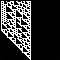
\includegraphics[scale=0.50]{../tex/images/CARule110}} & 108 
  														& \multicolumn{2}{c|}{\multirow{2}{*}{10}} \\ \cline{2-4}
  					 									& Rule30 (Unpalatable)& \parbox[c]{2.1em}{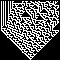
\includegraphics[scale=0.50]{../tex/images/CARule30}}  & 108 
  					 									& \multicolumn{2}{c|}{}\\ \hline
  \multirow{2}{*}{Reproduction} & Age Limit & \multicolumn{2}{c|}{100}  & \multicolumn{2}{c|}{500} \\ \cline{2-6}
  						 									& Interval  & \multicolumn{2}{c|}{1000} & \multicolumn{2}{c|}{1200} \\ \hline
  \multirow{2}{*}{Mutation Rate} & Pattern   & \multicolumn{2}{c|}{0.05} & \multicolumn{2}{c|}{\multirow{2}{*}{0.3}} \\ \cline{2-4}
  						 									 & Genome    & \multicolumn{2}{c|}{0.5}  & \multicolumn{2}{c|}{} \\ \hline
  Demise Age	 									 & \multicolumn{3}{c|}{2000}							& \multicolumn{2}{c|}{2500} \\ \hline
  Minimum Attack Age						 & \multicolumn{3}{c|}{} 						    & \multicolumn{2}{c|}{500} \\ \hline
  \multirow{2}{*}{\parbox{2cm}{Memory Configuration}} & \multicolumn{3}{c|}{} 					& Minimum & 2 \\ \cline{5-6}
   																			& \multicolumn{3}{c|}{} 					& Maximum & 10 \\ \hline  
\end{tabular}
\caption{Agent configuration of 2 prey species}
\label{tab:config-table-2-prey}
\end{table}

The set of parameters in table \ref{tab:config-table-2-prey} were carefully selected to be the initial condition for this run of the simulation. This test has been done with two sets of prey species with very different Cellular Automata pattern and with opposite palatability and equal population. To control reproduction of the prey species their age limit has been set to 100 iterations into the time the species were alive. And the reproduction interval was set to 1000 iterations.

Pattern mutation rate has been set to a minimal level of 0.05 as by increasing this variable it is possible to increase the size of the number of mimicry rings present in the simulation. The genome mutation rate controls the rate at which genome of the child prey species will deviate from their parents. As mentioned earlier the genome mutation rate has been separated from the pattern mutation rate to bring more control to the number of mimicry rings generated.

Prey demise age has been kept to 2000 iterations while predator demise age is set to 2500. But in the later experiments predator demise age has been increased to 5000 iterations. Predators in this simulation generate selection pressure for the evolution of mimicry. So the longer a predator is present in the simulation it will be making intelligent decisions in term of selecting which prey species to consume and which one to avoid. But with the current rate of demise for predator we were able to create successful mimetic population of prey species as we will see in the analysis in the following results.

Initial population of predator species has been set to 10 which is in accordance with the prey population in the simulation. The reason for such low number of predator is, unlike prey species which are consumed by predators, there is no cause for the predator species to die accept their natural cause of death, that is to reach their demise age. So predator population can explode very easily. That is why their population is controlled in a restrictive manner with the help of high reproduction age limit and reproduction age interval.

The memory configuration size for predators is a very interesting parameter. The minimum memory size is directly associated with the number of prey species with which we initiate the simulation. Otherwise evolution of mimicry is not observed. As mentioned in table \ref{tab:predator-control-parameters} the minimum memory size is the number of prey species predator would consume before starting to make decisive consumption of prey species. After the initial birth of a predator and when the minimum attack age is crossed, it starts consuming prey species present in its vicinity without making any judgment. At this point its memory size is zero. As long as the minimum memory size is not reached predators will blindly consume prey species and insert their CA pattern and associated palatability into its Hopfield memory bank. No later than the minimum memory size has been reached, predators will start making intelligent decision about consuming its prey species. When catching a prey if its memory tells that it is palatable, it will consume that prey. Otherwise if memory recognizes it to be unpalatable predator will certainly let it go.

Now as we know the behavior of Hopfield memory, a recognition result will always be achieved depending on the similarity of the patterns stored in memory. So when minimum memory size has been reached the predator will always make a decision based on the similarity of the prey pattern currently captured and the patterns stored in memory.

% Put the image
\begin{figure}[h]
	\centering
	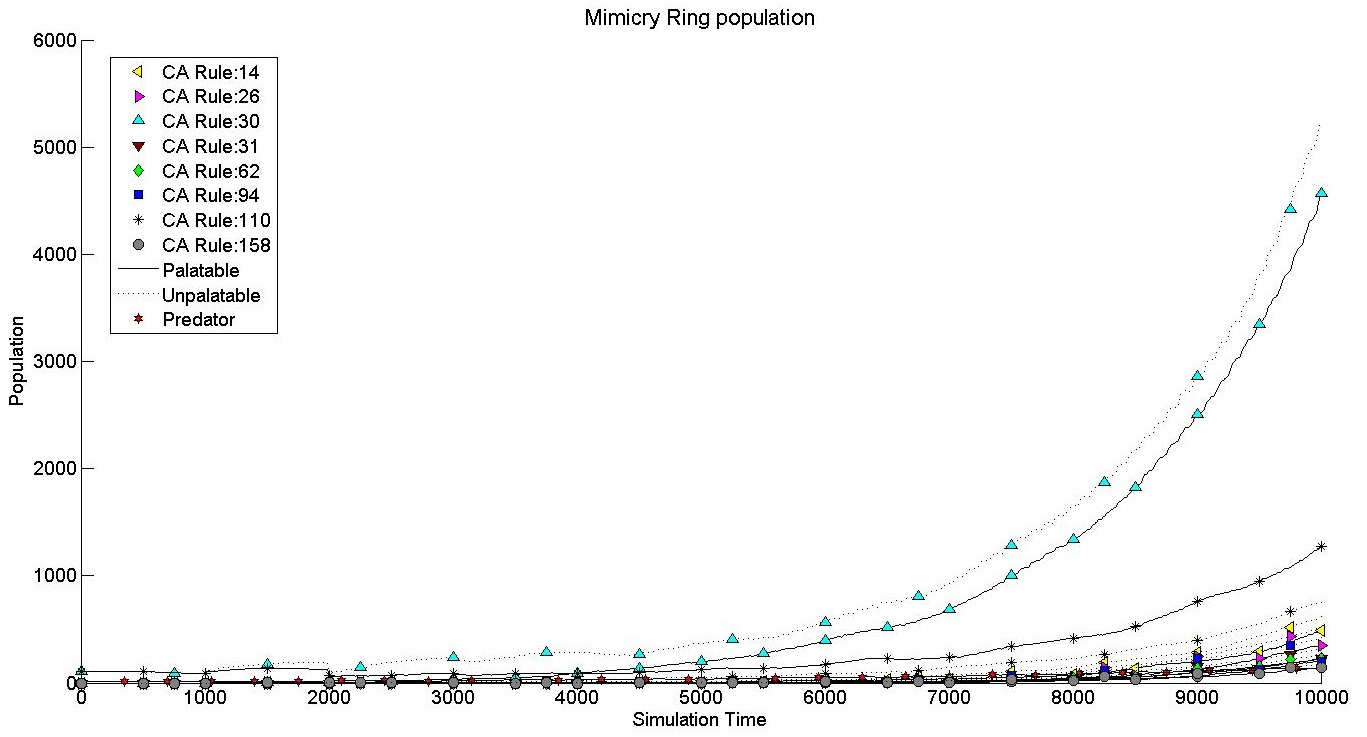
\includegraphics[width=0.5\textwidth]{../tex/images/simTime10k-2Prey}
	\caption[Population distribution of mimicry rings (2 prey species, 10k iterations)]{Population distribution of mimicry rings, initialized with 2 prey species, 10k iterations}
	\label{fig:plot-2-prey}
\end{figure}

The plot in Figure \ref{fig:plot-2-prey} is simulation time verses prey population after running it for 10000 iterations. With the initial configuration in the above table we can observe that multiple rings of prey population have been created. Two prey species are considered to be in a ring if their CA pattern have a Hamming distance within 10 bits. This parameter is mentioned in table \ref{tab:ring-report-control-parameters}. Population of palatable species has been represented with line curve while population of unpalatable species has been presented with dotted curve. Different signs of squares, triangles and diamonds have been used to distinguish between species of prey population. The simulation was initiated with two prey species having CA rule of 30 and 110 and being palatable and unpalatable consecutively.

\begin{figure}[h]
	\centering
	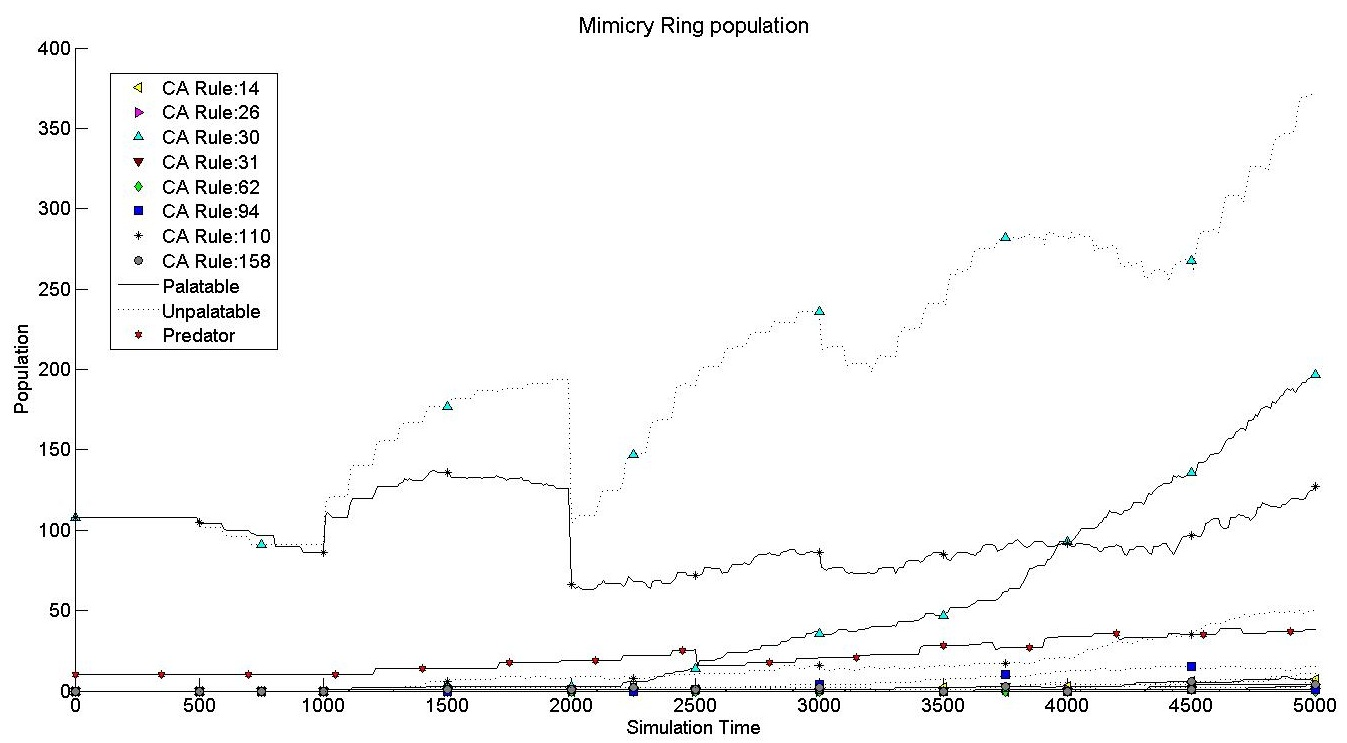
\includegraphics[width=0.5\textwidth]{../tex/images/simTime5k-2Prey}
	\caption[Population distribution of mimicry rings (2 prey species, 5k iterations)]{Population distribution of mimicry rings, initialized with 2 prey species, 5k iterations.}
	\label{fig:plot-2-prey-5k}
\end{figure}

The plot of figure \ref{fig:plot-2-prey-5k} is from the same experiment as of figure \ref{fig:plot-2-prey}, but only up to 5000 iterations. By closely observing the graph of figure \ref{fig:plot-2-prey-5k}, we could see the population of two species have started dropping at around time 500 when the initial predator population reaches the maturity for consuming prey species (effect of the parameter `Minimum Attack Age' from table \ref{tab:config-table-2-prey}). At around time 1000 the prey population starts reproducing as the population increases (controlled by `Reproduction Age Limit' from table \ref{tab:config-table-2-prey}). At the same time different other species of prey gets to be born with mutated CA patterns. There is a straight drop of prey population at time 2000, when all the prey species with which the simulation was initialized come to its demise age (controlled by `Prey Demise Age' at table \ref{tab:config-table-2-prey}). Over time the population of CA Rule 30 dominates the population (figure \ref{fig:plot-2-prey}) as most predators recognize it as unpalatable. Similarly a palatable population of CA Rule 30 or within the same ring of palatable species starts rising, while at one point overlaps the population of CA Rule 110 (Time: 4000 approx.). CA Rule 110 was initialized as a set of palatable species.

We can observe from the above result that the evolution of mimicry has taken effect. A population of mimics were successfully able to exceed the population of other prey species, and the reason being, avoidance by predators of prey pattern similar to unpalatable ones. We can conclude that Batesian mimicry has taken effect in the simulation.

%Put the number of rings picture:
\begin{figure}[h]
	\centering
	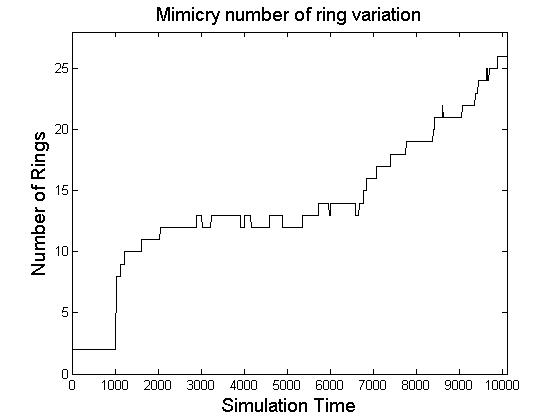
\includegraphics[width=0.5\textwidth]{../tex/images/ringSize10k-2Prey}
	\caption[Number of mimicry rings (2 prey species)]{Number of mimicry rings, initialized with 2 prey species.}
	\label{fig:ringSize10k-2Prey}
\end{figure}

Observing from figure \ref{fig:ringSize10k-2Prey} the number of rings in this simulation makes a slow increase from 2 at the initial configuration to 27 rings at the end of 10000 iterations. A small change in CA genetic representation can have a very large effect in terms of the phenotype of the pattern with which the prey is represented. For example if we take a look at the set of pattern genotype with very different phenotype in table \ref{tab:diff-in-pattern}.

%CARule table
\begin{table}[h]
\centering
\setlength\tabcolsep{2pt}
\begin{tabular}{|l|c|c|c|}
  \hline
  CA Rule & \(60 \equiv 00111100\) & \(61 \equiv 00111101\) & \(62 \equiv 00111110 \) \\ \hline
  Pattern & \parbox[c]{2.1em}{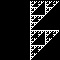
\includegraphics[scale=0.50]{../tex/images/CARule60}} 
  				& \parbox[c]{2.1em}{
\includegraphics[scale=0.50]{../tex/images/CARule61}} 
  				& \parbox[c]{2.1em}{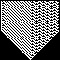
\includegraphics[scale=0.50]{../tex/images/CARule62}}\\
  \hline
\end{tabular}
\caption{Difference in prey pattern genotype and phenotype}
\label{tab:diff-in-pattern}
\end{table}

All the patterns in table \ref{tab:diff-in-pattern} have a genetic bit difference of 1. So by a single mutation there can be three different set of phenotype for a child organism from its parent. This is largely the reason for the increased number of mimicry rings created in the simulation. Only the 8 most populous rings are presented in the graphs with population verses simulation time.

\begin{figure}[h]
	\centering
	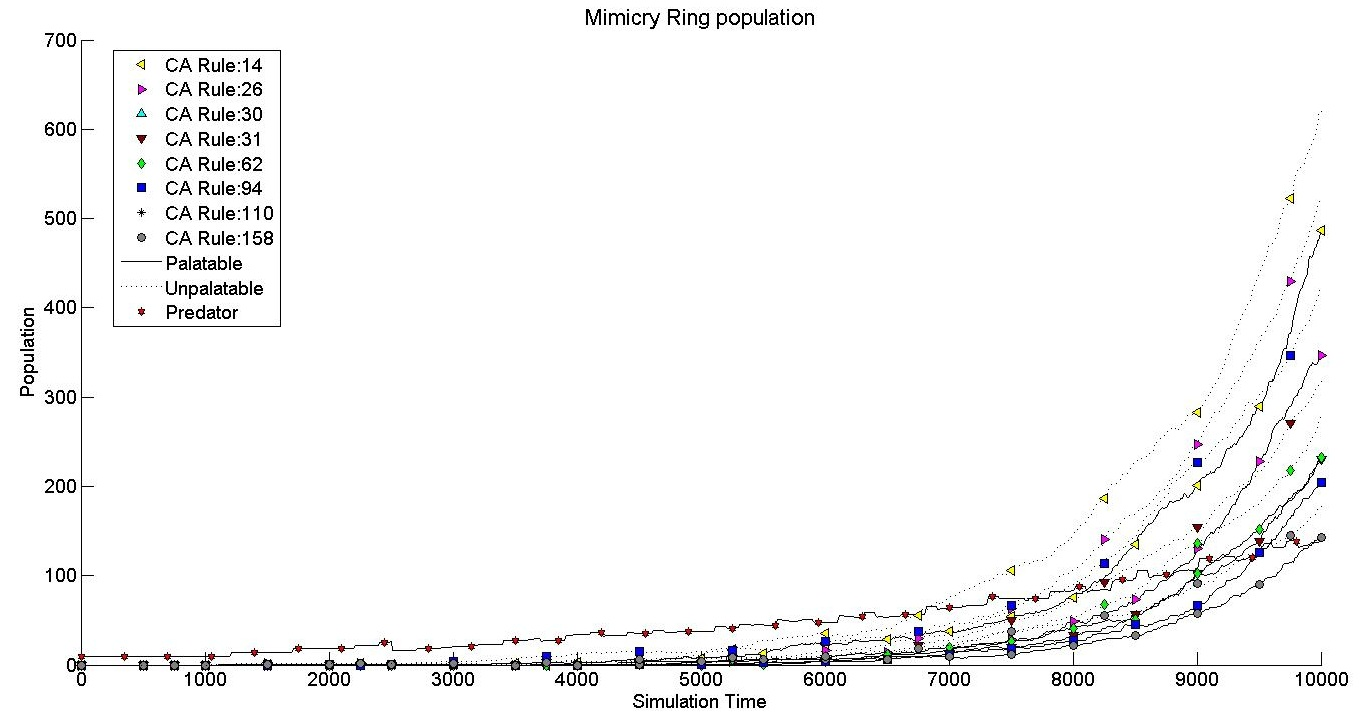
\includegraphics[width=0.5\textwidth]{../tex/images/simTime10k-2Prey-generated-prey}
	\caption[Population distribution of generated mimicry rings (2 prey species)]{Population distribution of generated mimicry rings, initialized with 2 prey species.}
	\label{fig:plot-2-prey-generated-prey}
\end{figure}

Figure \ref{fig:plot-2-prey-generated-prey} is the same experimental data of figure \ref{fig:plot-2-prey} but with only the newly generated ring of prey species. The initialized dominant population of CA rule 110 and 30, both palatable and unpalatable has been eliminated from this graph to observe the newly created rings. In this plot, among the population of new patterns the unpalatable ones dominate (CA Rule 14, 26, 94). Also the palatable counterpart of the unpalatable population is increasing their number. Species with \textsl{un-mimicked} palatable pattern is very few in number.

The screen shot in figure \ref{fig:screenshot-simTime7600-2-prey} is for one instance of time of the simulation. The red agents are predators while the black agents with different textured patterns are the prey species. According to their behavior most of the prey species are flocking together in a group while also being chased by the predators, whose sole purpose is to consume prey species. 

%Screenshot of the simulation
\begin{figure}[h]
	\centering
	\label{fig:screenshot-simTime7600-2-prey}
	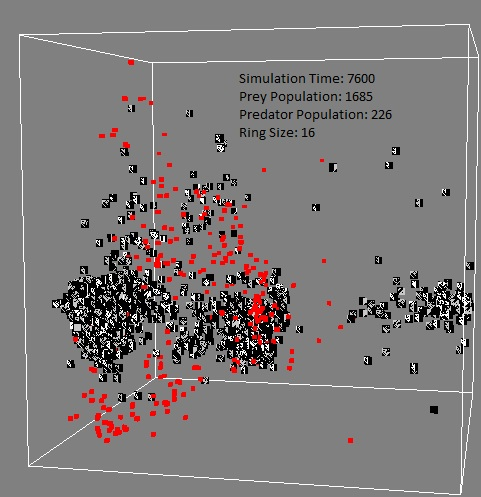
\includegraphics[width=0.5\textwidth]{../tex/images/simTime7600}
	\caption[Graphical representation of the model (simulation time: 7600)]{Graphical representation of the model, simulation time: 7600.}
\end{figure}

\subsection{Initial population with six prey species}
\label{subsec:init-conf-6-prey}
\begin{table}[h]
\centering
\setlength\tabcolsep{2pt}
\begin{tabular}{| p{2cm} | p{1.5cm} | p{1cm} | p{.5cm} | p{1.5cm} | p{.5cm} |}
  \hline
   														&\multicolumn{3}{c|}{Prey configuration} 																	
   														& \multicolumn{2}{c|}{\parbox{2cm}{Predator \\ configuration}} \\ \hline
  \multirow{6}{*}{Population} & Rule110 (Palatable) & \parbox[c]{2.1em}{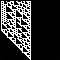
\includegraphics[scale=0.50]{../tex/images/CARule110}} 
  																									& 150 & \multicolumn{2}{c|}{\multirow{6}{*}{30}} \\ \cline{2-4}
  					 									& Rule30  (Unpalatable)& \parbox[c]{2.1em}{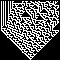
\includegraphics[scale=0.50]{../tex/images/CARule30}}  
  					 																				& 150 & \multicolumn{2}{c|}{}\\ \cline{2-4}
  					 									& Rule55  (Palatable)& \parbox[c]{2.1em}{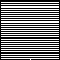
\includegraphics[scale=0.50]{../tex/images/CARule55}}    
  					 																				& 150 & \multicolumn{2}{c|}{}\\ \cline{2-4}
  					 									& Rule190 (Unpalatable)& \parbox[c]{2.1em}{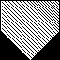
\includegraphics[scale=0.50]{../tex/images/CARule190}} 
  					 																				& 150 & \multicolumn{2}{c|}{}\\ \cline{2-4}
  					 									& Rule57  (Palatable)& \parbox[c]{2.1em}{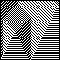
\includegraphics[scale=0.50]{../tex/images/CARule57}}    
  					 																				& 150 & \multicolumn{2}{c|}{}\\ \cline{2-4}
  					 									& Rule105 (Unpalatable)& \parbox[c]{2.1em}{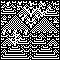
\includegraphics[scale=0.50]{../tex/images/CARule105}}& 150 & \multicolumn{2}{c|}{}\\ \hline
  \multirow{2}{*}{Reproduction} & Age Limit & \multicolumn{2}{c|}{100}  & \multicolumn{2}{c|}{500} \\ \cline{2-6}
  						 									& Interval  & \multicolumn{2}{c|}{1000} & \multicolumn{2}{c|}{2000} \\ \hline
  \multirow{2}{*}{Mutation Rate} & Pattern   & \multicolumn{2}{c|}{0.05} & \multicolumn{2}{c|}{\multirow{2}{*}{0.3}} \\ \cline{2-4}
  						 									 & Genome    & \multicolumn{2}{c|}{0.5}  & \multicolumn{2}{c|}{} \\ \hline
  Demise Age	 									 & \multicolumn{3}{c|}{2000}							& \multicolumn{2}{c|}{7000} \\ \hline
  Minimum Attack Age						 & \multicolumn{3}{c|}{} 						    & \multicolumn{2}{c|}{500} \\ \hline
  \multirow{2}{*}{\parbox{2cm}{Memory Configuration}} & \multicolumn{3}{c|}{} 					& Minimum & 6 \\ \cline{5-6}
   																			& \multicolumn{3}{c|}{} 					& Maximum & 10 \\ \hline  
\end{tabular}
\caption{Agent configuration of 6 prey species.}
\label{tab:config-table-6-prey}
\end{table}

To evaluate the simulation at a more complex level we increase the prey population to 900, consisting of 6 different species with very different pattern configuration. To boost predator-prey interaction we also increase the number of predator population to 30. Predator reproduction interval has been set comparatively lower in this simulation to 2000 iterations. As the initial population of prey species is very high, over time we are expecting even larger number of prey species. If predator population does not increase at similar rate there might be a prey population explosion were predator will have no effect on providing selection pressure for the evolution of mimicry. So that is why predator population control parameter has been set to this level. For memory configuration, the minimum number is set to 6, meaning the predator will have to store 6 different prey pattern configuration before starting to make intelligent decision about consuming them. As previously mentioned this number is always set in accordance with the initial number of different prey configuration. 

\begin{figure}[h]
	\centering
	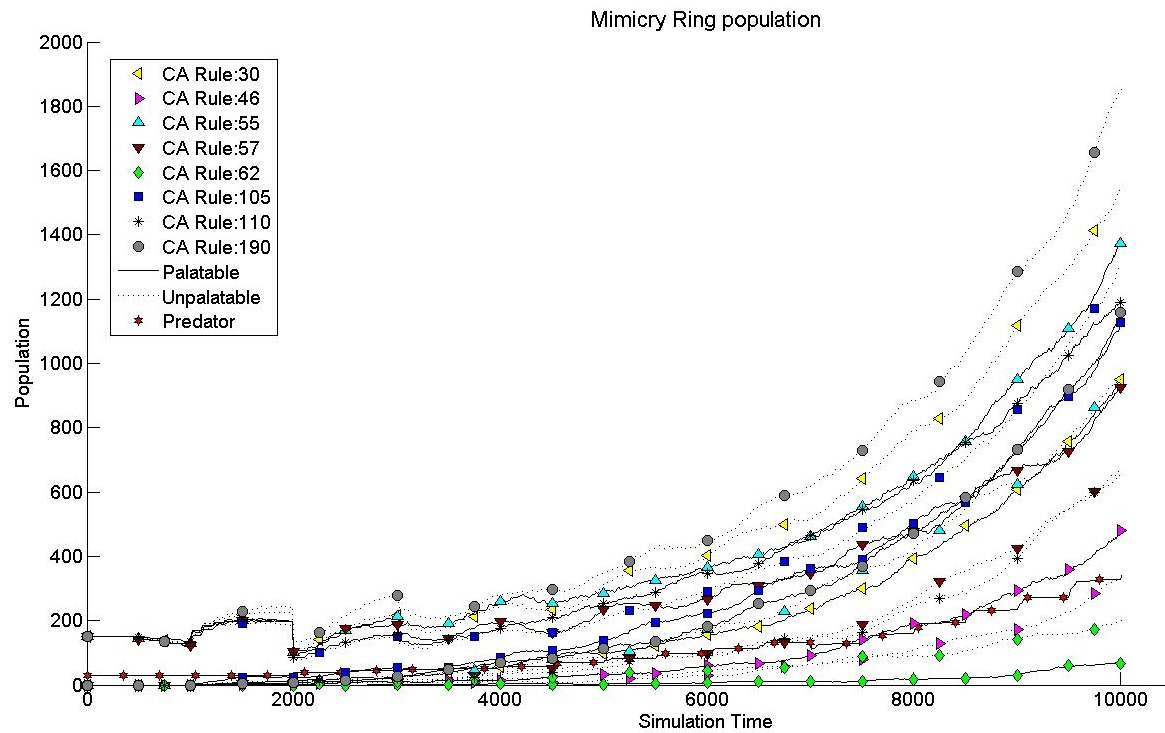
\includegraphics[width=0.5\textwidth]{../tex/images/simTime10k-6Prey}
	\caption[Population distribution of mimicry rings (6 prey species)]{Population distribution of mimicry rings, initialized with 6 prey species.}
	\label{fig:plot-6-prey}
\end{figure}

With the above set of parameters we receive the plot of figure \ref{fig:plot-6-prey}. An enormous diversity of species can be observed from this experiment. In addition to the six prey species with which the simulation starts, the total number of mimicry rings reach nearly 50. Observing the top 8 as presented in the plot of figure \ref{fig:plot-6-prey}, effects of Batesian mimicry is obvious. Unpalatable CA Rule 190 and 30 dominates the population. Similarly unpalatable CA Rule 105 is also dominant. But after 10000 iterations CA Rule 55 seems to have higher population than 105 even though 55 is a \textsl{palatable} set of species. This anomaly could be the reason for storing large number of patterns in the predator Hopfiled memory. As we know that the number of patterns stored in Hopfiled network is inversely proportional to its recognition rate. In this simulation memory size is controlled by the `Maximum Memory Configuration' which is set to 10 in table \ref{tab:config-table-6-prey}. In this experiment, the value of `Minimum Memory Configuration' is 6, which is rather a large number. So there could be possibility of wrong recognition by Hopfield memory. Then again this phenomenon is common if we consider behavior of predators in nature. It is definitely hard for a single predator to memorize multiple poisonous patterns and because of which Mullerian mimicry takes an effect as mentioned in section \ref{subsec:mullerian-mimicry}.

\begin{figure}[h]
	\centering
	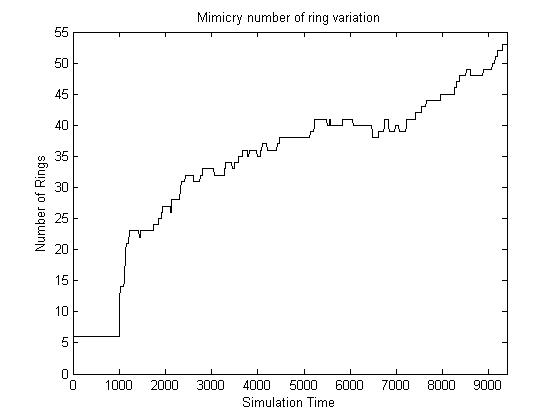
\includegraphics[width=0.5\textwidth]{../tex/images/ringSize10k-6Prey}
	\caption[Number of mimicry rings (6 prey species)]{Number of mimicry rings, initialized with 6 prey species.}
	\label{fig:ringSize10k-6-Prey}
\end{figure}

\subsection{Initial configuration with only unpalatable species}
\label{subsec:init-conf-only-unp}
\begin{table}[h]
\centering
\setlength\tabcolsep{2pt}
\begin{tabular}{| p{2cm} | p{1.5cm} | p{1cm} | p{.5cm} | p{1.5cm} | p{.5cm} |}
  \hline
   														&\multicolumn{3}{c|}{Prey configuration} 																	
   														& \multicolumn{2}{c|}{\parbox{2cm}{Predator \\ configuration}} \\ \hline
  \multirow{4}{*}{Population} & Rule110 (Unpalatable) & \parbox[c]{2.1em}{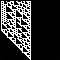
\includegraphics[scale=0.50]{../tex/images/CARule110}} 
  																									& 150 & \multicolumn{2}{c|}{\multirow{4}{*}{20}} \\ \cline{2-4}
  					 									& Rule30  (Unpalatable)& \parbox[c]{2.1em}{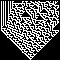
\includegraphics[scale=0.50]{../tex/images/CARule30}}  
  					 																				& 150 & \multicolumn{2}{c|}{}\\ \cline{2-4}
  					 									& Rule55  (Unpalatable)& \parbox[c]{2.1em}{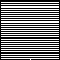
\includegraphics[scale=0.50]{../tex/images/CARule55}}    
  					 																				& 150 & \multicolumn{2}{c|}{}\\ \cline{2-4}
  					 									& Rule190 (Unpalatable)& \parbox[c]{2.1em}{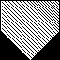
\includegraphics[scale=0.50]{../tex/images/CARule190}}& 150 & \multicolumn{2}{c|}{}\\ \hline
  \multirow{2}{*}{Reproduction} & Age Limit & \multicolumn{2}{c|}{100}  & \multicolumn{2}{c|}{500} \\ \cline{2-6}
  						 									& Interval  & \multicolumn{2}{c|}{1000} & \multicolumn{2}{c|}{2000} \\ \hline
  \multirow{2}{*}{Mutation Rate} & Pattern   & \multicolumn{2}{c|}{0.05} & \multicolumn{2}{c|}{\multirow{2}{*}{0.3}} \\ \cline{2-4}
  						 									 & Genome    & \multicolumn{2}{c|}{0.5}  & \multicolumn{2}{c|}{} \\ \hline
  Demise Age	 									 & \multicolumn{3}{c|}{2000}							& \multicolumn{2}{c|}{5000} \\ \hline
  Minimum Attack Age						 & \multicolumn{3}{c|}{} 						    & \multicolumn{2}{c|}{500} \\ \hline
  \multirow{2}{*}{\parbox{2cm}{Memory Configuration}} & \multicolumn{3}{c|}{} 					& Minimum & 4 \\ \cline{5-6}
   																			& \multicolumn{3}{c|}{} 					& Maximum & 10 \\ \hline  
\end{tabular}
\caption{Agent configuration of 4 prey species all unpalatable.}
\label{tab:config-table-4-prey-unpalatable}
\end{table}

To further observe the effects of mimicry ring we initialize the simulation with all unpalatable prey species. After finding different anomalous behavior of predator recognition capability in section \ref{subsec:init-conf-6-prey} for increased number of diverse prey species; for this experiment the initial number of species have been reduced from six to four. As explained earlier the minimum memory configuration is also set to four in accordance to the initial number of prey species. Rest of the parameters remain quite unchanged.

\begin{figure}[h]
	\centering
	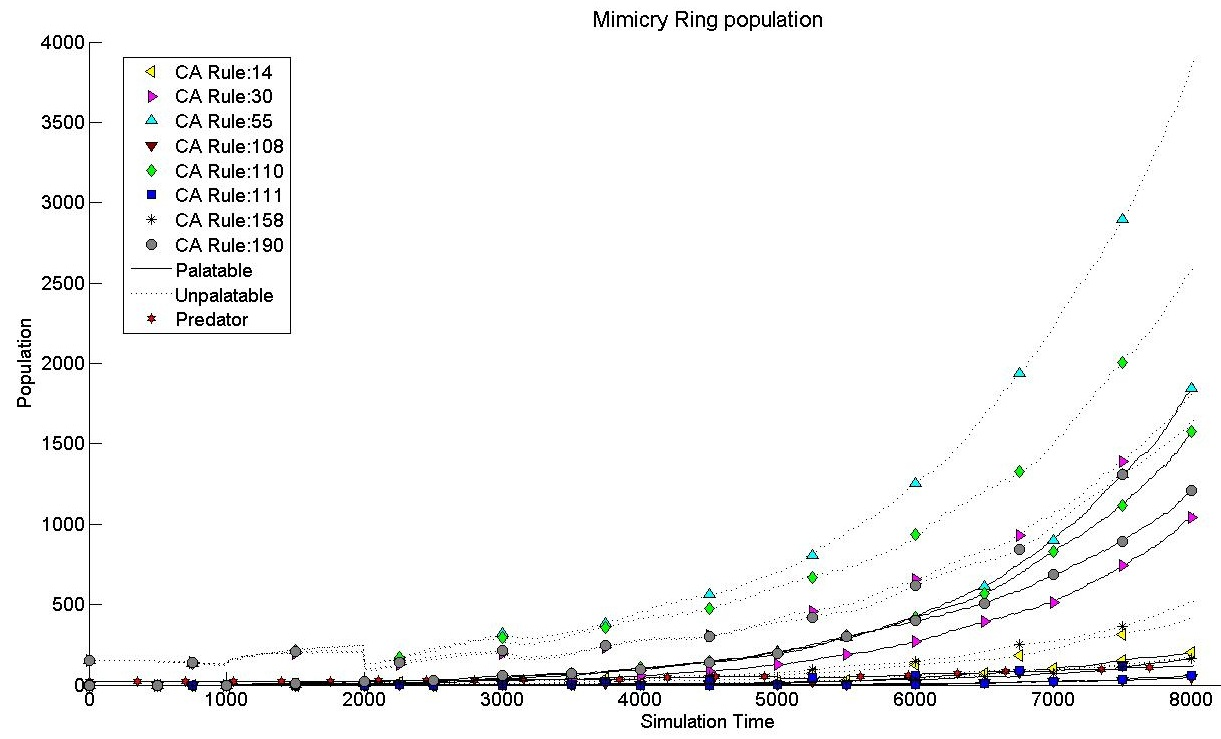
\includegraphics[width=0.5\textwidth]{../tex/images/simTime8k-4Prey-unp}
	\caption[Population distribution of mimicry rings(4 prey species all unpalatable)]{Population distribution of mimicry rings, initialized with 4 prey species all unpalatable.}
	\label{fig:plot-4-prey-unp}
\end{figure}

The results according to figure \ref{fig:plot-4-prey-unp} are much expected. The population of unpalatable species have prevailed. After nearly 8000 iterations we can see unpalatable species of CA rule 55, 110, 30 and 190 have prevailed with the most population. All of their palatable counter parts are also increasing their population deceiving the predators. We observe the effect of the simulation up to 8000 iterations instead of 10000 as the total number of prey species increases at an enormous rate in this simulation within very short period of time. As most of the species are unpalatable, predators mostly do not get the opportunity to consume, causing a much lower prey death rate. 

\begin{figure}[h]
	\centering
	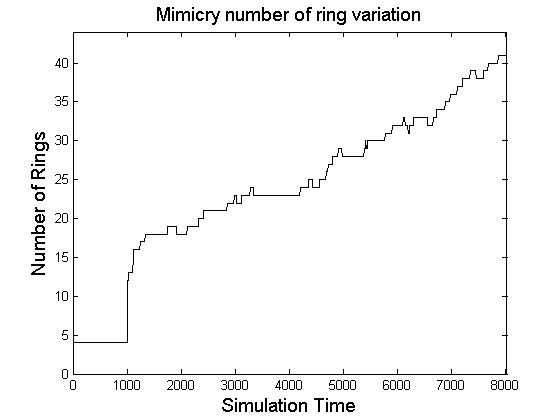
\includegraphics[width=0.5\textwidth]{../tex/images/ringSize8k-4Prey-unp}
	\caption[Number of mimicry rings (4 prey species all unpalatable)]{Number of mimicry rings, initialized with 4 prey species all unpalatable.}
	\label{fig:ringSize10k-4-Prey-unp}
\end{figure}

This experiment is an ideal scenario for observing Mullerian mimicry. As mentioned in section \ref{subsec:mullerian-mimicry}, Mullerian mimicry occurs between multiple species of unpalatable prey population. From the second work of Franks and Noble \citep{franks2003} mentioned in section \ref{subsubsec:models-by-frank-and-noble}, we note that multiple Mullerian mimicry rings are expected to converge into one large ring through the evolutionary process of punctuated equilibrium. But in this experiment as the predator's `Minimum Memory Configuration' is set to four, all predators have the capability to recognize four prey patterns before starting to make intelligent decision of consuming them. By setting `Minimum Memory Configuration' to one, also increasing `Predator Demise Age' to 7000 and decreasing predator's `Reproduction Age Interval' to 1500, we get the following plot. 

\begin{figure}[h]
	\centering
	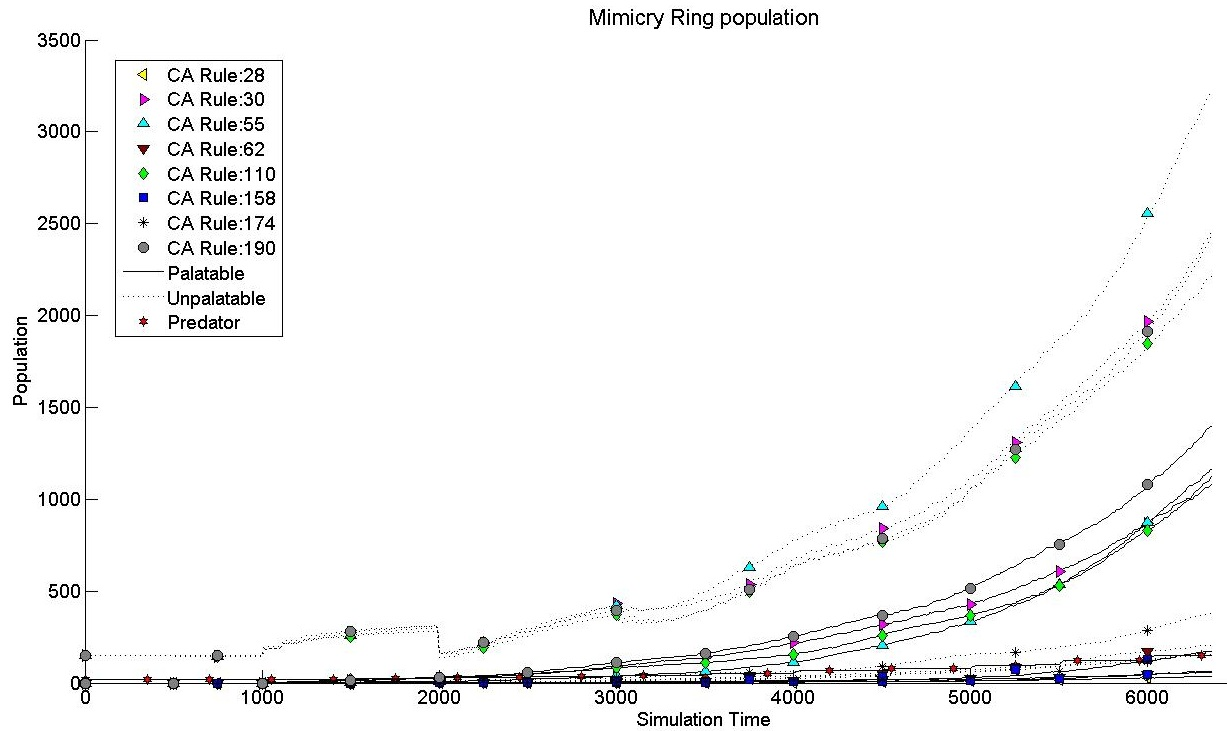
\includegraphics[width=0.5\textwidth]{../tex/images/simTime6k-4Prey-unp-1-mem}
	\caption[Population distribution of mimicry rings(4 prey, all unpalatable but reduced predator memory)]{Population distribution of mimicry rings, initialized with 4 prey species all unpalatable. Minimum Memory size reduced to one.}
	\label{fig:plot-4-prey-unp-1-mem}
\end{figure}

Running the simulation for 6000 iterations there was no sign for all prey population to converge into one large ring. As it can be observed in figure \ref{fig:plot-4-prey-unp-1-mem} all four unpalatable prey population have a very dominant presence in the simulation. Even though predator minimum memory has been reduced to only one pattern, different population of predators become familiar with different prey patterns, which results in the existence of multiple Mullerian mimicry ring instead of a single one.

\subsection{Initial configuration with only palatable species}
\label{subsec:init-only-palatable-species}

\begin{table}[h]
\centering
\setlength\tabcolsep{2pt}
\begin{tabular}{| p{2cm} | p{1.5cm} | p{1cm} | p{.5cm} | p{1.5cm} | p{.5cm} |}
  \hline
   														&\multicolumn{3}{c|}{Prey configuration} 																	
   														& \multicolumn{2}{c|}{\parbox{2cm}{Predator \\ configuration}} \\ \hline
  \multirow{4}{*}{Population} & Rule110 (Palatable) & \parbox[c]{2.1em}{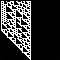
\includegraphics[scale=0.50]{../tex/images/CARule110}} 
  																									& 150 & \multicolumn{2}{c|}{\multirow{4}{*}{20}} \\ \cline{2-4}
  					 									& Rule30  (Palatable)& \parbox[c]{2.1em}{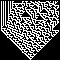
\includegraphics[scale=0.50]{../tex/images/CARule30}}  
  					 																				& 150 & \multicolumn{2}{c|}{}\\ \cline{2-4}
  					 									& Rule55  (Palatable)& \parbox[c]{2.1em}{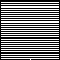
\includegraphics[scale=0.50]{../tex/images/CARule55}}    
  					 																				& 150 & \multicolumn{2}{c|}{}\\ \cline{2-4}
  					 									& Rule190 (Palatable)& \parbox[c]{2.1em}{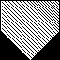
\includegraphics[scale=0.50]{../tex/images/CARule190}}& 150 & \multicolumn{2}{c|}{}\\ \hline
  \multirow{2}{*}{Reproduction} & Age Limit & \multicolumn{2}{c|}{100}  & \multicolumn{2}{c|}{500} \\ \cline{2-6}
  						 									& Interval  & \multicolumn{2}{c|}{1000} & \multicolumn{2}{c|}{2000} \\ \hline
  \multirow{2}{*}{Mutation Rate} & Pattern   & \multicolumn{2}{c|}{0.05} & \multicolumn{2}{c|}{\multirow{2}{*}{0.3}} \\ \cline{2-4}
  						 									 & Genome    & \multicolumn{2}{c|}{0.5}  & \multicolumn{2}{c|}{} \\ \hline
  Demise Age	 									 & \multicolumn{3}{c|}{2000}							& \multicolumn{2}{c|}{5000} \\ \hline
  Minimum Attack Age						 & \multicolumn{3}{c|}{} 						    & \multicolumn{2}{c|}{500} \\ \hline
  \multirow{2}{*}{\parbox{2cm}{Memory Configuration}} & \multicolumn{3}{c|}{} 					& Minimum & 4 \\ \cline{5-6}
   																			& \multicolumn{3}{c|}{} 					& Maximum & 10 \\ \hline  
\end{tabular}
\caption{Agent configuration of 4 prey species all palatable.}
\label{tab:config-table-4-prey-palatable}
\end{table}

The parameters for this simulation has been set exactly the same as in table \ref{tab:config-table-4-prey-unpalatable} except all the species are palatable at this point. All predator configuration has also been set to exactly same as before.

The results for the configuration in table \ref{tab:config-table-4-prey-palatable} can be observed in figure \ref{fig:plot-4-prey-p} where all population of prey species have reached its demise at nearly 7000 iterations. By analyzing details we can see, around simulation time 500 all population of species come to a steady downfall as at this point initial predator species reach its' age for consumption. Around simulation time 1000 all population of prey species start increasing steadily because they reach their maturity level of reproduction. At iteration time 2000 there is a sudden drop of prey population because the initial population of prey have reached its demise age at this point. By this time the population of unpalatable species mutated from the palatable ones start increasing, and slowly around time 7000 and onwards the entire population of prey come to its demise. Predator population, from the beginning of the simulation has taken a very dominant effect. As all the species are palatable, predator's consumption and reproduction rate is extremely high and it keep increasing in a geometric rate.

\begin{figure}[h]
	\centering
	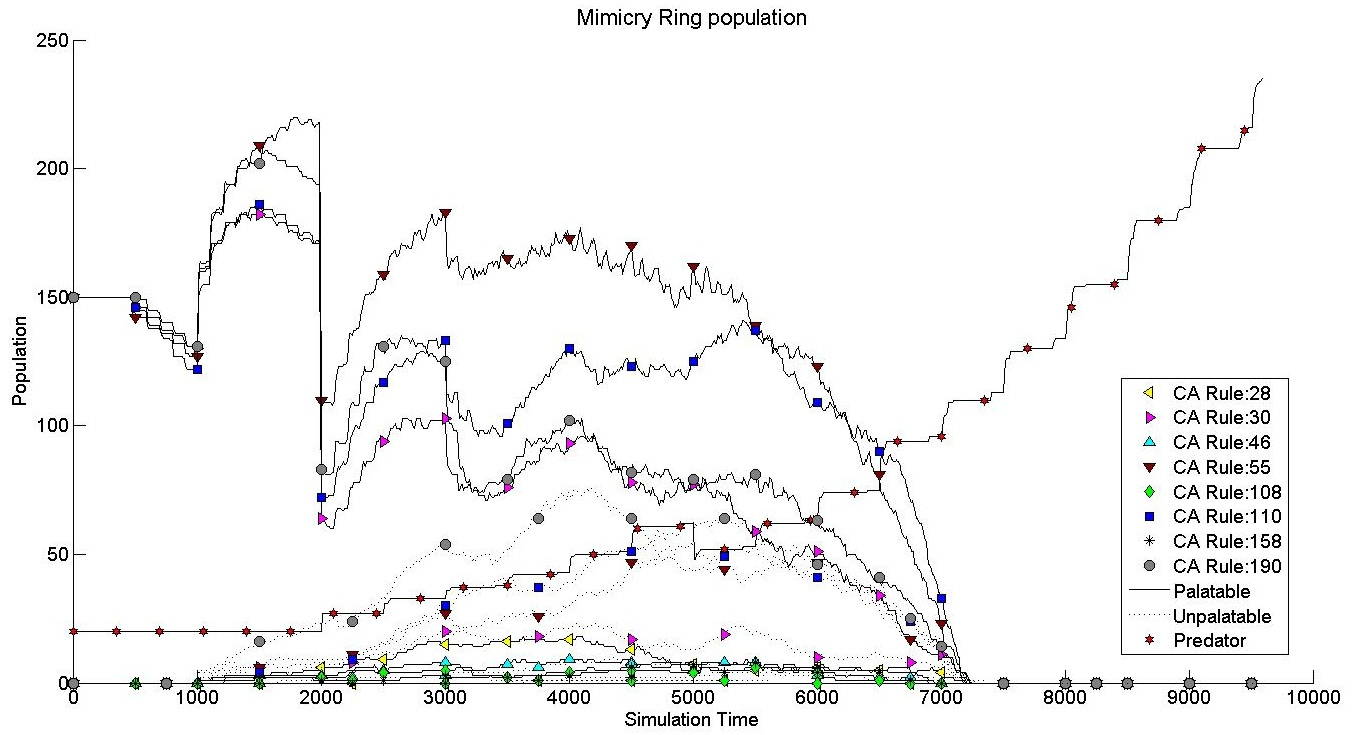
\includegraphics[width=0.5\textwidth]{../tex/images/simTime10k-4Prey-p}
	\caption[Population distribution of mimicry rings (4 prey species all palatable)]{Population distribution of mimicry rings, initialized with 4 prey species all palatable.}
	\label{fig:plot-4-prey-p}
\end{figure}

\begin{figure}[h]
	\centering
	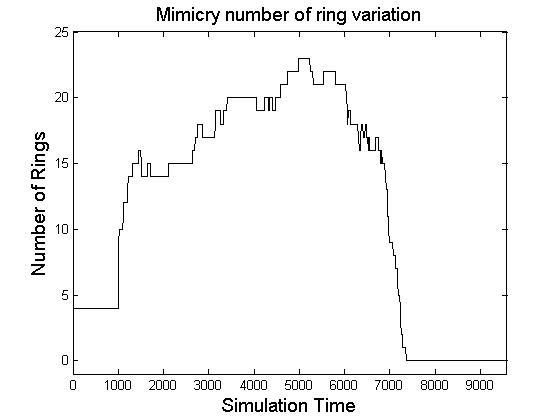
\includegraphics[width=0.5\textwidth]{../tex/images/ringSize10k-4Prey-p}
	\caption[Number of mimicry rings (4 prey species all palatable)]{Number of mimicry rings, initialized with 4 prey species all palatable.}
	\label{fig:ringSize8k-4-Prey-p}
\end{figure}

Observation of mimicry rings also tell us about the results we have seen in the plot of figure \ref{fig:plot-4-prey-p}. The number of rings keep increasing but comes to a sudden drop around simulation time 7000 and goes to zero.

\subsection{Analysis of Batesian Mimicry}
\label{subsec:result-batesian-mimicry}
For all possible initial conditions, Batesian mimicry has taken effect. It can be observed that for every ring of unpalatable species there is an existence of the palatable ring racing to reach the population count of its unpalatable counterpart. Also when the initial population starts with a set of only palatable species we can observe that the total population vanishes within very short period of time (section \ref{subsec:init-only-palatable-species}). This effect can be explained with the fact that the palatable population does not have any models to mimic, and it reaches extinction. So from this analysis it can be concluded that the model under discussion have successfully simulated the evolution of Batesian mimicry.

\subsection{Analysis of Mullerian Mimicry}
\label{subsec:result-mullerian-mimicry}
Effects of Mullerian mimicry can be observed best for the experiment in section \ref{subsec:init-conf-only-unp}. For that case, we initialized the model with 4 rings of unpalatable species with no palatable ones and after nearly 10K iterations, all of the initial unpalatable rings have survived with dominance. The cause of this behavior can be explained by the minimum number of patterns that each predator can store in memory, which was set to four. So this parameter was reduced to one to observe whether it is possible to converge all different unpalatable rings into one large ring, when predators are capable to memorizing only a single pattern. But as it turned out, the phenomena of ``a single large ring" does not occur because different predators recognize different patterns resulting in multiple divergent Mullerian mimicry rings. It can be concluded that our results are consistent with those of Franks and Noble (section \ref{subsubsec:models-by-frank-and-noble}), that multiple Mullerian mimics do not converge into one large ring.

\section{Conclusion}
\label{section:conclusion}
Analysis of the results tell us that we have successfully been able to simulate the evolution of mimicry. In addition to that, this model provides a more accurate simulation of the fascinating natural process of mimicry rings. Not only does this model simulates mimicry with the initialized population but also it provides possibility of creating diverse new rings and their shift in population. This model also verifies the theory of Turner in explaining the evolution of mimicry with punctuated equilibrium (section \ref{subsubsec:reflection-of-punctuated-equilibrium}) \citep{turner1988}.

If we consider the field of Artificial Life as a tool for biological inquiry then the model presented in this thesis was successful in terms of providing good insight in terms of understanding better the evolutionary process of mimicry as it happens in nature. As mentioned previously this model gives us verification of the theory of Turner in explaining the evolution of mimicry with punctuated equilibrium. Also it enforces findings from the work of Franks and Noble that multiple Mullerian mimics do not converge into one large ring.

If we consider Artificial Life as the study where we simulate natural processes to further extend capabilities in the field of computer science, then also this thesis is a success in making an appropriate emulation of the evolutionary process of mimicry. From the sections of \ref{subsec:result-batesian-mimicry} and \ref{subsec:result-mullerian-mimicry} we can conclude that the complex behavior of Batesian and Mullerian mimicry can be simulated with this model.

\bibliographystyle{apalike}
\bibliography{references}

\printglossaries
\phantomsection \label{acronyms}

\end{document}
